%%% UNIT 1
{
\setbeamertemplate{headline}{}
\setbeamertemplate{footline}{
  \begin{beamercolorbox}[wd=\paperwidth,ht=2.2ex,dp=1.5ex]{palette quaternary}
  \end{beamercolorbox}
  }
\begin{frame}[noframenumbering]
\frametitle{\DB{\huge{\textbf{$\blacksquare$ Unit 1}}}}
\myPause
 \begin{itemize}
 \item[] \LARGE{\MB{Foreword and prerequisites}}
 \item[] \vspace{-1mm}\LARGE{\MB{Introducing ``control''}}
 \item[] \vspace{-1mm}\LARGE{\MB{Terminology and first examples}}
 \item[] \vspace{-1mm}\LARGE{\MB{A quick visit to the zoo of control}}
 \item[] \vspace{-1mm}\LARGE{\MB{Dynamic systems -- an introduction}}
 \item[] \vspace{-1mm}\LARGE{\MB{Conclusions and discussion}}
 \end{itemize}
\end{frame}
}

\part{}

\section{Foreword and prerequisites}
\subsection{}

\begin{frame}
\frametitleTC{What we are going to do together}
\framesubtitleTC{in a nutshell}
\myPause
\begin{quote}
If you search the literature for ``control in computers'', you will find first that there is a lot of material, and then that the so-called ``PID'' controller is one of the most widely employed.\\
However, as we shall see, an incorrect use of that object can be as disastrous as a good one beneficial. Hence you need to understand and master the underlying principles, that is, the essentials of the systems and feedback control theory.\\
This activity will make you capable in the first place of using PID control knowledgeably, and as a by-product, will also teach you what a dynamic model of a system is.\\
In turn, this is useful for many purposes, including e.g. to detect\\
when a problem cannot be tackled with a PID, and thus you need\\
to learn more control, or ask for advice from a control specialist,\\
or both.
\end{quote}
\end{frame}

\begin{frame}
\frametitleTC{Prerequisites}
\framesubtitleTC{(1/3) mathematics}
\myPause
\begin{itemize}[<+-| alert@+>]
\item Basic knowledge of differential/integral calculus:
      \begin{itemize}[<.(1)->]
      \item limit (finite and infinite),
      \item derivative and integral in one variable.
      \end{itemize}
      \myPause
\item Complex numbers and operations on them.
\item Basic knowledge of matrix algebra:
      \begin{itemize}[<.(1)->]
      \item matrix operations,
      \item determinant, inverse,
      \item eigenvalues and eigenvectors.
      \end{itemize}
\end{itemize}
\end{frame}


\begin{frame}
\frametitleTC{Prerequisites}
\framesubtitleTC{(2/3) physics --- yes we do need a little bit for some examples}
\myPause
\begin{itemize}[<+-| alert@+>]
\item Mass balance: the time derivative of the mass $M$ contained in a volume\\
      (e.g., a tank) is the sum of the $n$ signed mass flowrates $w_i$ at the $n$ boundaries\\
      (e.g., pipes) of that volume, that is,
      \begin{displaymath}
       \frac{dM(t)}{dt} = \sum_{i=1}^n w_i(t).
      \end{displaymath}
\item Energy balance: the time derivative of the energy $E$ contained in a volume\\
      (e.g., a solid body) is the sum of the $n$ signed powers $q_i$ at the $n$\\
      boundaries (e.g., surfaces) of that volume, that is,
      \begin{displaymath}
       \frac{dE(t)}{dt} = \sum_{i=1}^n q_i(t).
      \end{displaymath}
\item We evidently take the convention ``positive means entering''.
\end{itemize}
\end{frame}

\begin{frame}
\frametitleTC{Prerequisites}
\framesubtitleTC{(3/3) physics --- yes we do need a little bit for some examples}
\myPause
\begin{itemize}[<+-| alert@+>]
\item Convective/conductive heat transfer: the power $q_{ab}$ transferred form a body at temperature $T_a$
      to another at temperature $T_b$ is proportional by a \emph{thermal conductance} $G_{ab}$ to the temperature
      difference, that is,
      \begin{displaymath}
       q_{ab}(t) = G_{ab} \left( T_a(t)-T_b(t) \right).
      \end{displaymath}
\item Anticipation: later on we shall see more balances of the \emph{dynamic} type, i.e.,\\
      taking the form``the time derivative of something equals the sum\\
      of something else''.
\item You may be surprised how frequent these are in computing systems,\\
      hence how many different problems can be treated uniformly.
\end{itemize}
\end{frame}


\section{Introducing ``control''}
\subsection{}

\begin{frame}
\frametitleTC{The word ``control'' in the Merriam-Webster dictionary$^*$
              \blfootnote{\small{$^*$\texttt{https://www.merriam-webster.com/dictionary/control}}}}
\framesubtitleTC{(1/3) verb} 
\myPause
\emph{transitive verb}
\begin{tabular}{lll}
 \bf{1} & \bf{a} & archaic: to check, test, or verify by evidence or experiments \\
        & \bf{b} & :to incorporate suitable controls in \\
        &        & \textbf{//} \emph{a controlled experiment} \\
 \bf{2} & \bf{a} & :to exercise restraining or directing influence over: REGULATE \\
        &        & \textbf{//} \emph{control one's anger} \\
        & \bf{b} & :to have power over: RULE \\
        &        & \textbf{//} \emph{A single company controls the industry.} \\
        & \bf{c} & :to reduce the incidence or severity of especially to innocuous levels \\
        &        & \textbf{//} \emph{control an insect population} \\
        &        & \textbf{//} \emph{control a disease} \\
\end{tabular}\\
\vspace{2mm}\emph{intransitive verb}\\
\begin{tabular}{lll}
 :to incorporate controls in an experiment or study -- used with for \\
 \textbf{//} \emph{control for socioeconomic differences}\\
\end{tabular}
\end{frame}

\begin{frame}
\frametitleTC{The word ``control'' in the Merriam-Webster dictionary}
\framesubtitleTC{(2/3) noun} 
\myPause
\begin{tabular}{lll}
 \bf{1} & \bf{a} & :an act or instance of controlling \\
        &        & also: power or authority to guide or manage \\
        &        & \textbf{//} \emph{He took control of the family business.} \\
        & \bf{b} & :skill in the use of a tool, instrument, technique, or artistic medium \\
        &        & \textbf{//} \emph{a singer's control of her voice} \\
        & \bf{c} & :the regulation of economic activity especially by government directive \\
        &        & -- usually used in plural \\
        &        & \textbf{//} \emph{price controls} \\
        &        & \textbf{//} \emph{rent controls} \\
        & \bf{d} & :the ability of a baseball pitcher to control the location of a pitch \\
        &        & within the strike zone \\
 \bf{2} &        & :RESTRAINT, RESERVE \\
        &        & \textbf{//} \emph{exercised control of his passions}
\end{tabular}
\end{frame}

\begin{frame}
\frametitleTC{The word ``control'' in the Merriam-Webster dictionary}
\framesubtitleTC{(3/3) noun, cont'd} 
\myPause
\begin{tabular}{lll}
 \bf{3} & \multicolumn{2}{l}{:one that controls: such as} \\
        & \bf{a} & \textbf{(1)} :an experiment in which the subjects are treated as in a parallel \\
        &        &  experiment except for omission of the procedure or agent under test and which \\
        &        &  is used as a standard of comparison in judging experimental effects\vspace{1mm} \\
        &        & -- called also \emph{control experiment} \\
        &        & \textbf{(2)} :one (such as an organism, culture, or group) that is part of a control \\
        & \bf{b} & a device or mechanism used to regulate or guide the operation of a machine,\\
        &        & apparatus, or system \\
        &        & \textbf{//} \emph{the controls of the aircraft} \\
        & \bf{c} & an organization that directs a spaceflight \\
        &        & \textbf{//} \emph{mission control} \\
        & \bf{d} & a personality or spirit believed to actuate the utterances or\\
        &        & performances of a spiritualist medium \\
 \bf{4} & \multicolumn{2}{l}{or less commonly Control: CONTROL KEY}
\end{tabular}
\end{frame}

\begin{frame}
\frametitleTC{The word is prone to being misunderstood}
\framesubtitleTC{Just a couple of examples} 
\myPause
\begin{itemize}[<+-| alert@+>]
\item Many synonyms (most dangerous ones for us in bold):
      \begin{itemize}
      \item[] bridle, \textbf{check}, constrain, contain, curb, govern, hold, inhibit, \\
              keep, \textbf{measure}, pull in, regulate, rein (in), restrain,\\
              rule, tame,...
      \end{itemize}
\item Many meanings depending on the viewpoint.
\item[] \vspace{-1.5mm}For example, the controls of an aircraft ``regulate or guide'' its operation.
\item[] \vspace{-0.75mm}Fine. So what kind of object/entity do we mean here for ``controls''?
      \begin{itemize}
      \item The knobs, levers and so forth that the pilot manoeuvres?
      \item ...or the autopilot computer with its software?
      \item ...or the ailerons, the rudder and the like?
      \item ...or the compound of all of these?
      \end{itemize}
      \myPause
\item \vfill We definitely need to state our terminology and notation precisely.
\end{itemize}
\end{frame}


\begin{frame}
\frametitleTC{Our definition}
\framesubtitleTC{Take 1 -- for now mostly intuitive, we shall be progressively more precise} 
\myPause
\begin{quote}
 \begin{center}
  \Large{Control is making something behave\\
         as close as possible to how you want it to behave,\\ \myPause
         most often despite there can be other actions besides yours,\\ \myPause
         and also despite you have only a partial knowledge\\
         of the phenomena you are acting upon, \\ \myPause
         hence even the effect of your own actions\\
         may be not entirely predictable.}
 \end{center}
\end{quote}
\end{frame}

\begin{frame}\mccz
\frametitleTC{Why a \underline{theory} for systems and control?}
\framesubtitleTC{} 
\myPause
\begin{quote}
 \begin{center}
  \only<2 | handout:0>{\vspace{-0.4mm}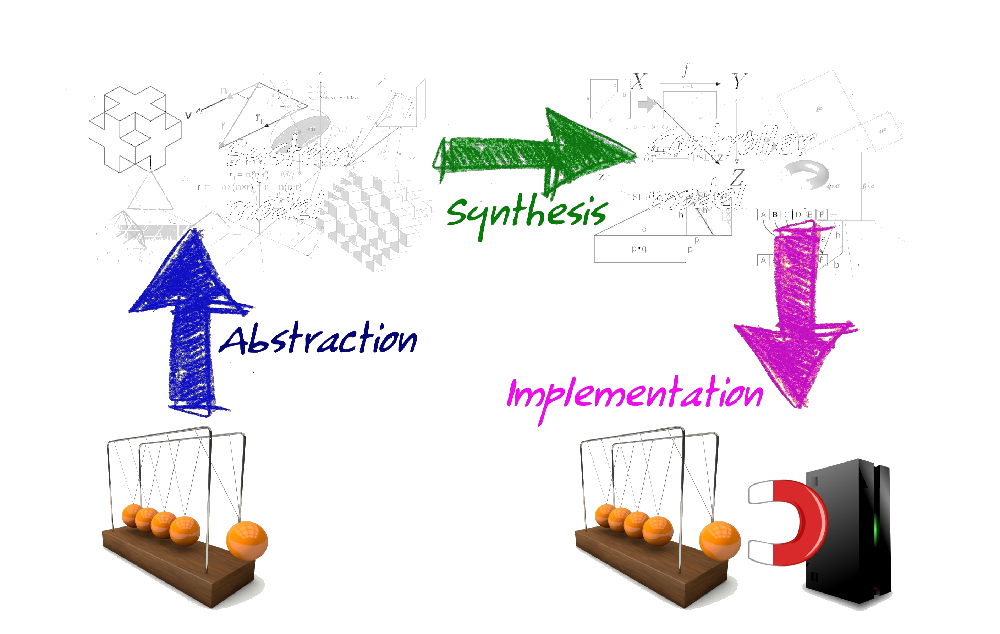
\includegraphics[width=0.85\columnwidth]{./Unit-01/img/RoleOfModels-1_cc0.png}}
  \only<3 | handout:0>{\vspace{-0.4mm}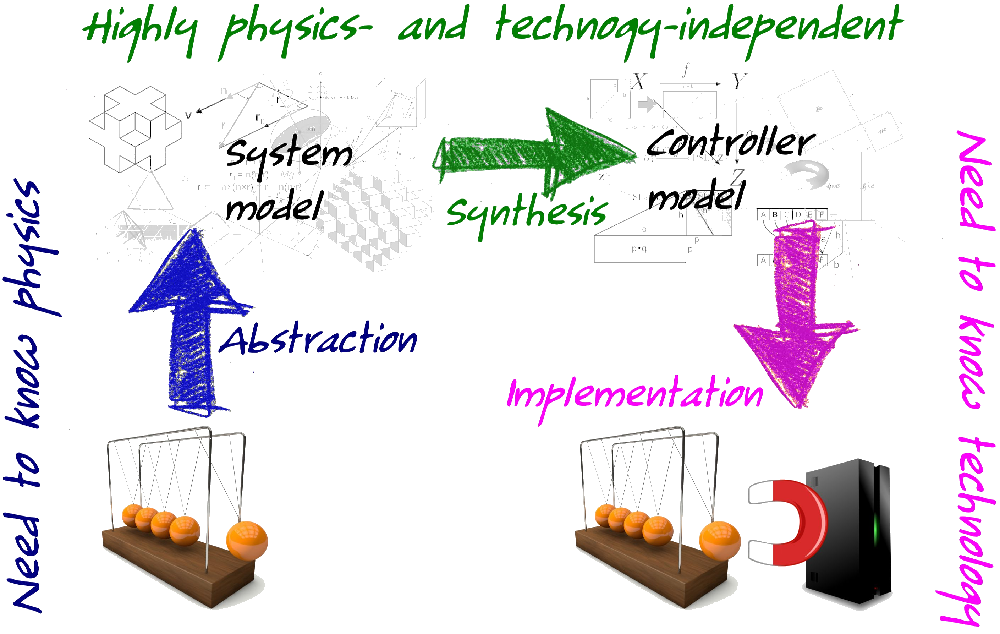
\includegraphics[width=0.85\columnwidth]{./Unit-01/img/RoleOfModels-2_cc0.png}}
  \only<4            >{\vspace{-0.4mm}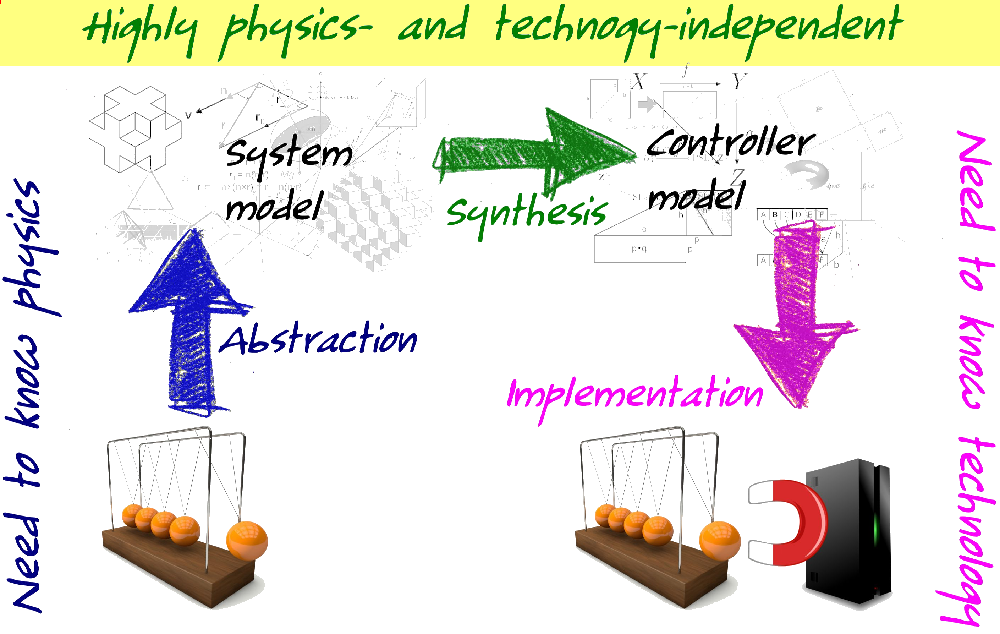
\includegraphics[width=0.85\columnwidth]{./Unit-01/img/RoleOfModels-3_cc0.png}}
 \end{center}
\end{quote}
\end{frame}


\section{Terminology and first examples}
\subsection{}

\begin{frame}
\frametitleTC{Terminology}
\framesubtitleTC{(1/2)}
\myPause
 \begin{itemize}[<+-| alert@+>]
 \item \TC{System} -- when required to avoid ambiguity, \TC{\underline{controlled} system:}
       \begin{itemize}[<+-| alert@+>]
       \item[] the object or phenomenon to be governed
       \item[] (a vehicle, the thermal behaviour of a building,...).
       \end{itemize}
 \item \TC{Requirements} or \TC{objectives:}
       \begin{itemize}[<+-| alert@+>]
       \item[] what you want the system to do\\
       \item[] (cruise as close as possible to 50 km/h, keep temperature between 18$^{\circ}$C\\
                and 21$^{\circ}$C in all rooms,...)
       \end{itemize}
 \item \TC{Controls} or \TC{control actions} or simply \TC{actions:}
       \begin{itemize}[<+-| alert@+>]
       \item[] what is done to the system with the purpose of fulfilling the requirements
       \item[] (act on the gas/brakes, modulate fuel flowrate to heater,\\
                operate fan coils,...).
       \end{itemize}
 \item \TC{Outcomes:}
       \begin{itemize}[<+-| alert@+>]
       \item[] the actual behaviour of the system
       \item[] (real speed and temperature behaviour over time,...).
       \end{itemize}
 \end{itemize}
\end{frame}

\begin{frame}
\frametitleTC{Terminology}
\framesubtitleTC{(2/2)}
\myPause
 \begin{itemize}[<+-| alert@+>]
 \item \TC{Disturbances:}
       \begin{itemize}[<+-| alert@+>]
       \item[] anything that affects the outcomes and cannot be manipulated, but possibly sensed
       \item[] (road slope, wind, vehicle load, weather, room occupancy,...);
       \item[] in other words, actions from the environment to which the system must be resilient.
       \end{itemize}
 \item \TC{Sensors:}
       \begin{itemize}[<+-| alert@+>]
       \item[] the entities that gather information from the system
       \item[] (tacho/accelerometer, GPS, inside/outside temperature sensors,...).
       \end{itemize}
 \item \TC{Actuators:}
       \begin{itemize}[<+-| alert@+>]
       \item[] the entities that act on the system to exert the actions
       \item[] (engine, brakes, burners, pumps, valves,...).
       \end{itemize}
 \item \TC{Controllers:}
       \begin{itemize}[<+-| alert@+>]
       \item[] the entities that determine the actions given the information\\
               deemed relevant\\
       \item[] (the object of your design).
       \end{itemize}
 \end{itemize}
\end{frame}

\begin{frame}
\frametitleTC{Remarks}
\framesubtitleTC{}
\myPause
 \begin{itemize}[<+-| alert@+>]
 \item Quite often we can talk about a control \TC{objective} in terms of a \TC{signal}\\
       following another one.
 \item In the case we use to say that
       \begin{itemize}[<+-| alert@+>]
       \item we have a \TC{controlled variable} (e.g., the speed of a vehicle)
       \item and want it to follow a \TC{set point} or \TC{reference} signal (e.g., go from 0 to 100 km/h
             linearly in 10 seconds).
       \end{itemize}
 \item Also, quite often our action can be viewed as setting a variable (e.g., the gas\\
       valve opening in the 0--100\% range); we call such a variable\\
       the \TC{control signal}.
 \item Consistently, we can often represent exogenous actions (e.g., wind\\
       speed and directions) that we called \TC{disturbances}, as signals.
 \end{itemize}
\end{frame}

\begin{frame}
\frametitleTC{Remarks}
\framesubtitleTC{}
\myPause
 \begin{itemize}[<+-| alert@+>]
 \item You are probably thinking that in the computer world the situation just sketched is hardly ever encountered.
 \item The objection seems in fact reasonable, as the entities one manages in computers are far more
       heterogeneous than mere numbers varying over time.
 \item \vfill Nonetheless hold on; you will discover that on the contrary, much more computer-related problems
       than one expects, can be formulated in terms\\ of \TC{set point following} and/or \TC{disturbance rejection}.
 \item In the end, learning systems and control is learning a new kind\\
       of abstraction.
 \end{itemize}
\end{frame}



\section{The control zoo}
\subsection{}

\begin{frame}\mccz
\frametitleTC{A first, quick visit to the zoo of control}
\myPause
 \begin{columns}
  \column[T]{0.20\textwidth}
   \only<2->{
\includegraphics[height=6cm]{./Unit-01/img/ZenWhale_cc0.jpg}}
  \column[T]{0.70\textwidth}
   \begin{quote}
    \begin{small}
     \onslide<3->{Now the various species of whales need some sort of popular comprehensive classification,
                  if only an easy outline one for the present, hereafter to be filled in all its departments
                  by subsequent labourers. As no better man advances to take this matter in hand, I hereupon
                  offer my own poor endeavours.\\
                  I promise nothing complete; because any human thing supposed to be complete, must for that
                  very reason infallibly be faulty. I shall not pretend to a minute anatomical description
                  of the various species, or -- in this place at least -- to much of any description.\\
                  My object here is simply to project the draught\\
                  of a systematisation of Cetology. I am the\\
                  architect, not the builder.\\
                  \vspace{1mm}$\qquad\qquad\qquad\;\;\;\;$H. Melville, Moby Dick, XXXII
                  }
    \end{small}
   \end{quote}
 \end{columns}
\end{frame}

\begin{frame}
\frametitleTC{A very simple control taxonomy -- axis 1}
\framesubtitleTC{What information is used by the controller (sensors and actuators not drawn for simplicity)}
\myPause
 \begin{itemize}[<+-| alert@+>]
 \item Requirements and possibly disturbances\\
       $\Rightarrow$ \TC{open-loop} control, possibly with \TC{disturbance compensation}:
       \begin{center}
        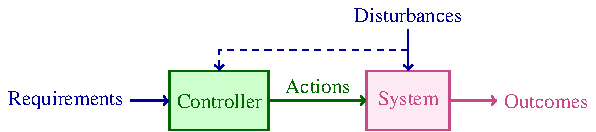
\includegraphics[width=0.60\columnwidth]{./Unit-01/img/Taxonomy-OpenLoop-scheme.pdf}
       \end{center}
 \item Requirements, \underline{system output(s)} and possibly disturbances\\
       $\Rightarrow$ \TC{closed-loop} or \TC{feedback} control, possibly with \TC{disturbance compensation}:
       \begin{center}
        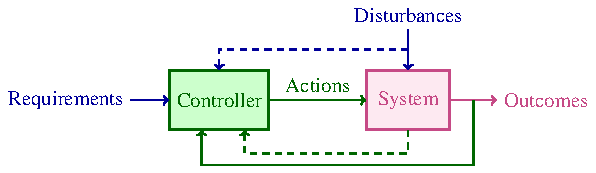
\includegraphics[width=0.60\columnwidth]{./Unit-01/img/Taxonomy-ClosedLoop-scheme.pdf}
       \end{center}
 \end{itemize}
\end{frame}

\begin{frame}\mccz
\frametitleTC{A very simple control taxonomy -- axis 2}
\framesubtitleTC{When the controller determines the control action}
\myPause
 \begin{columns}
  \column[T]{0.25\textwidth}
   \only<2 | handout:0>{\centering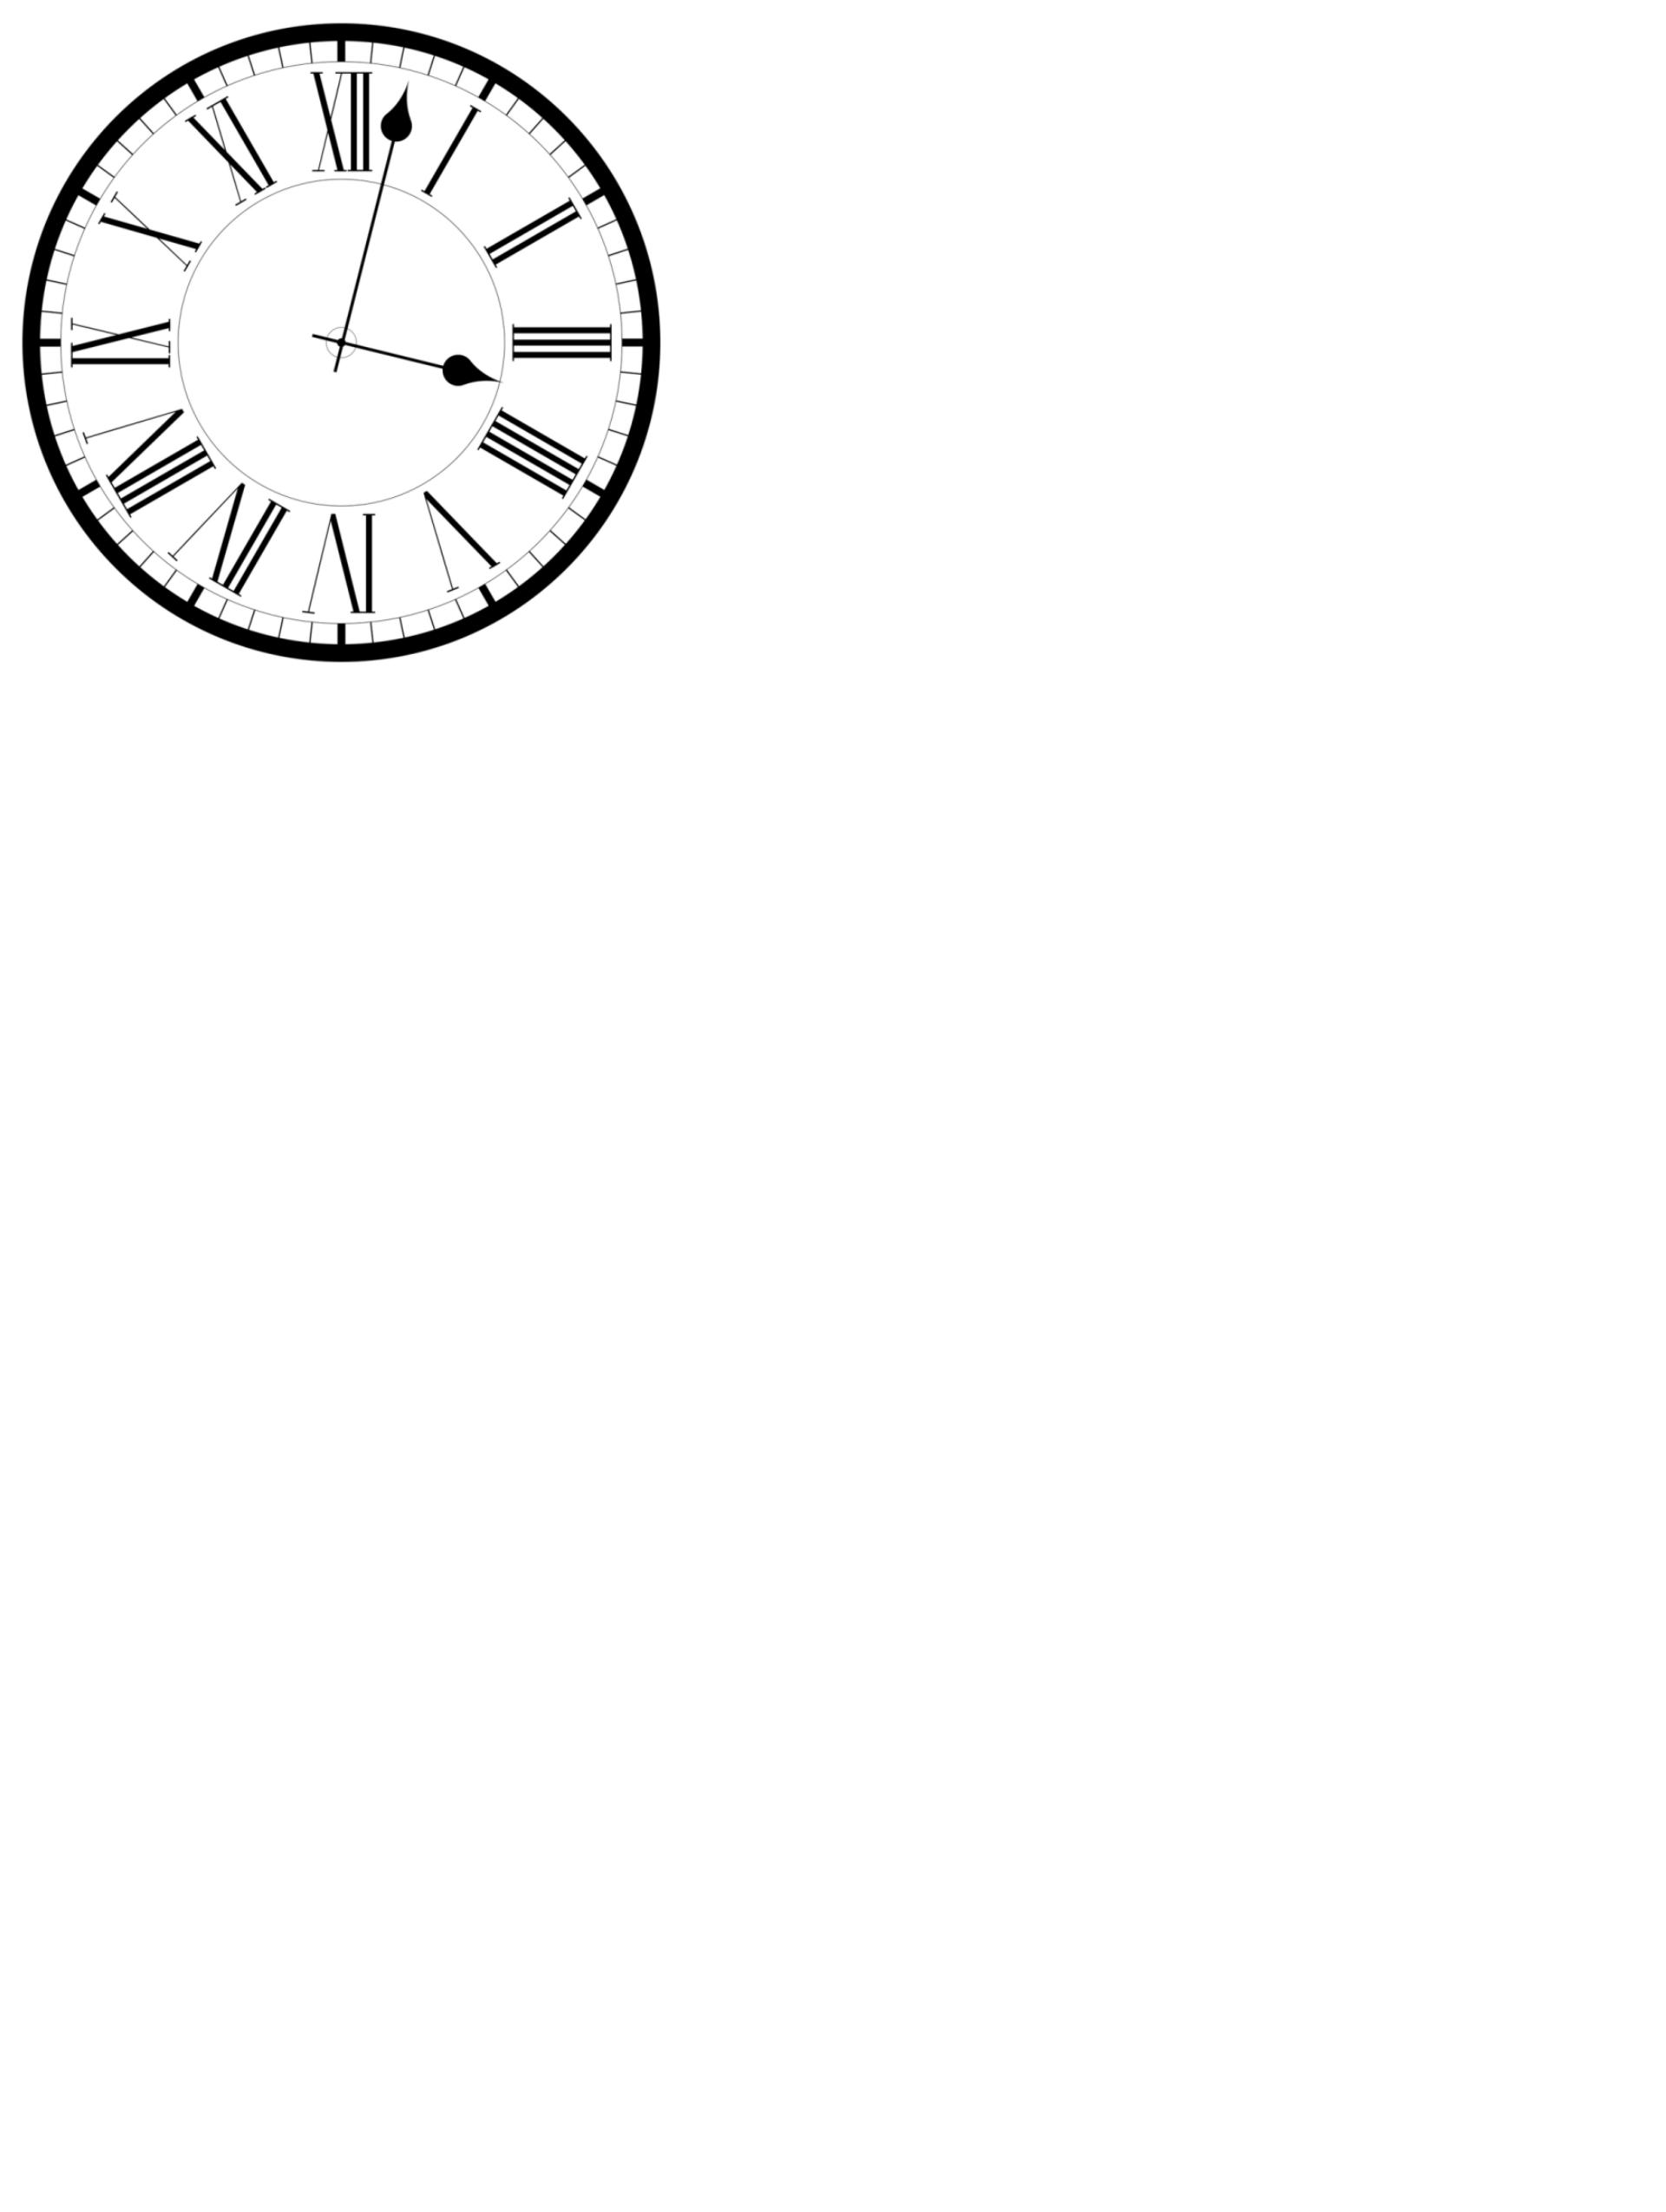
\includegraphics[height=5.5cm]{./Unit-01/img/Taxonomy-When-1_cc0.jpg}}%
   \only<3 | handout:0>{\centering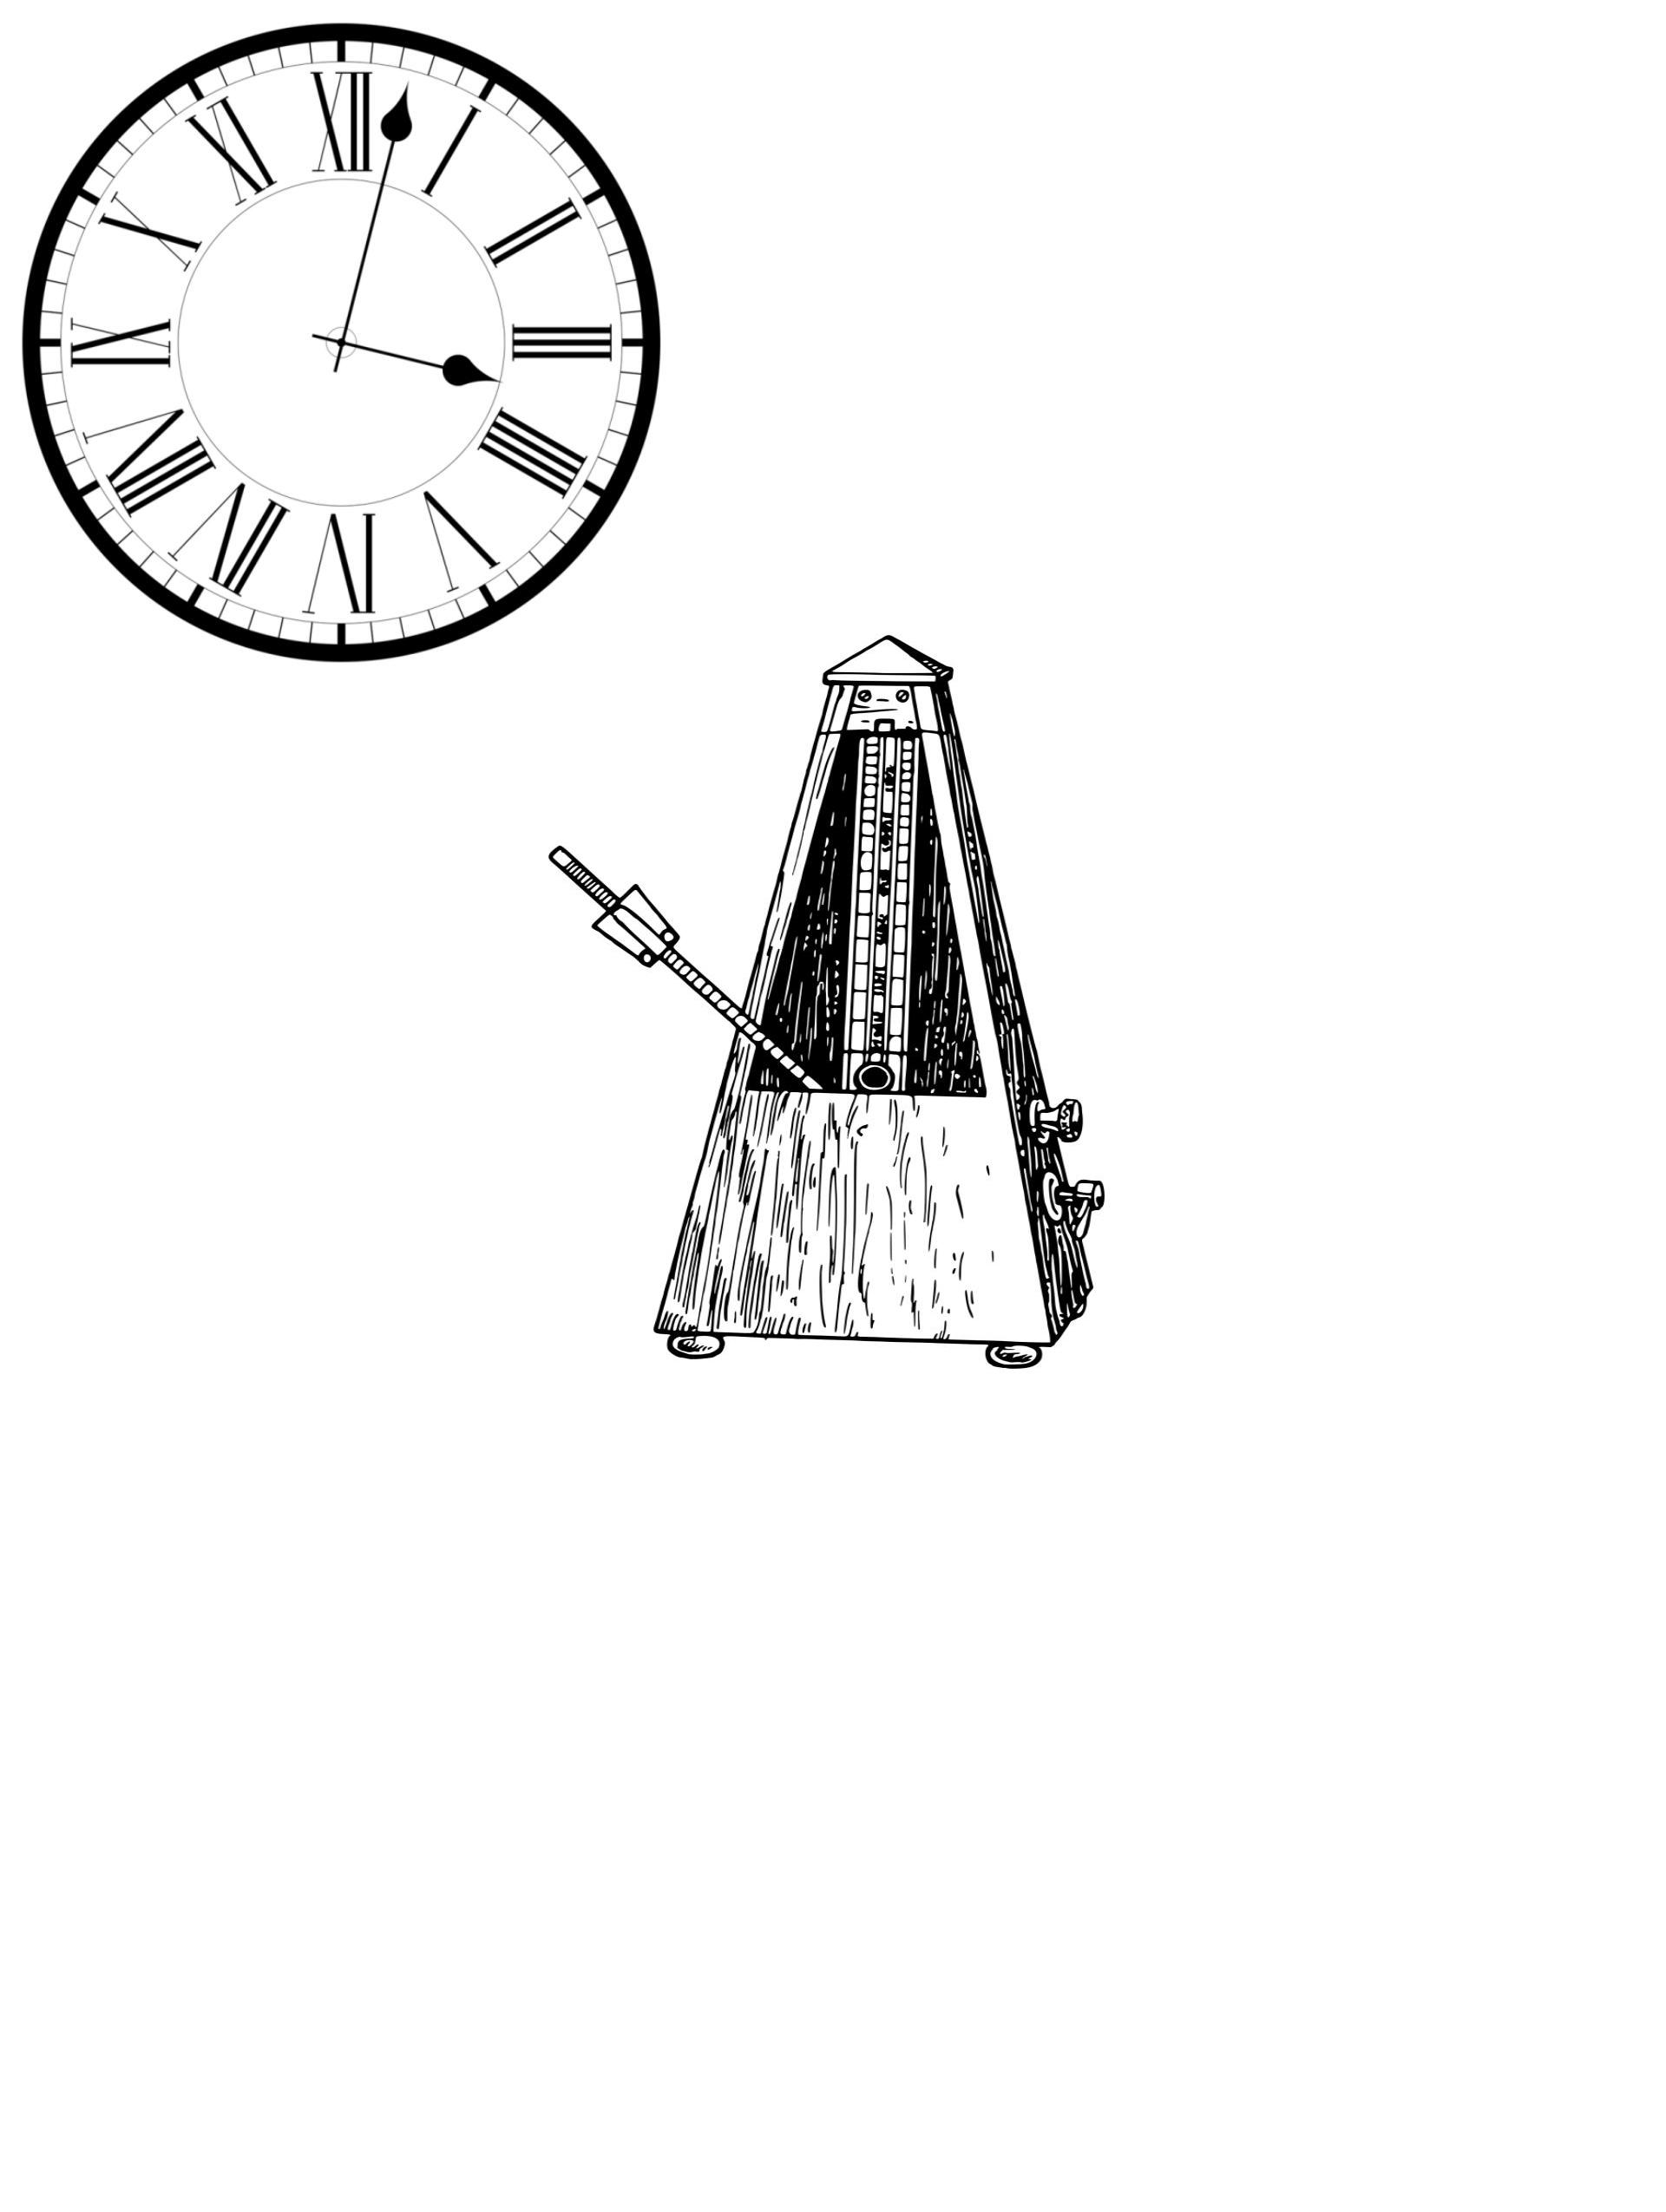
\includegraphics[height=5.5cm]{./Unit-01/img/Taxonomy-When-2_cc0.jpg}}%
   \only<4-           >{\centering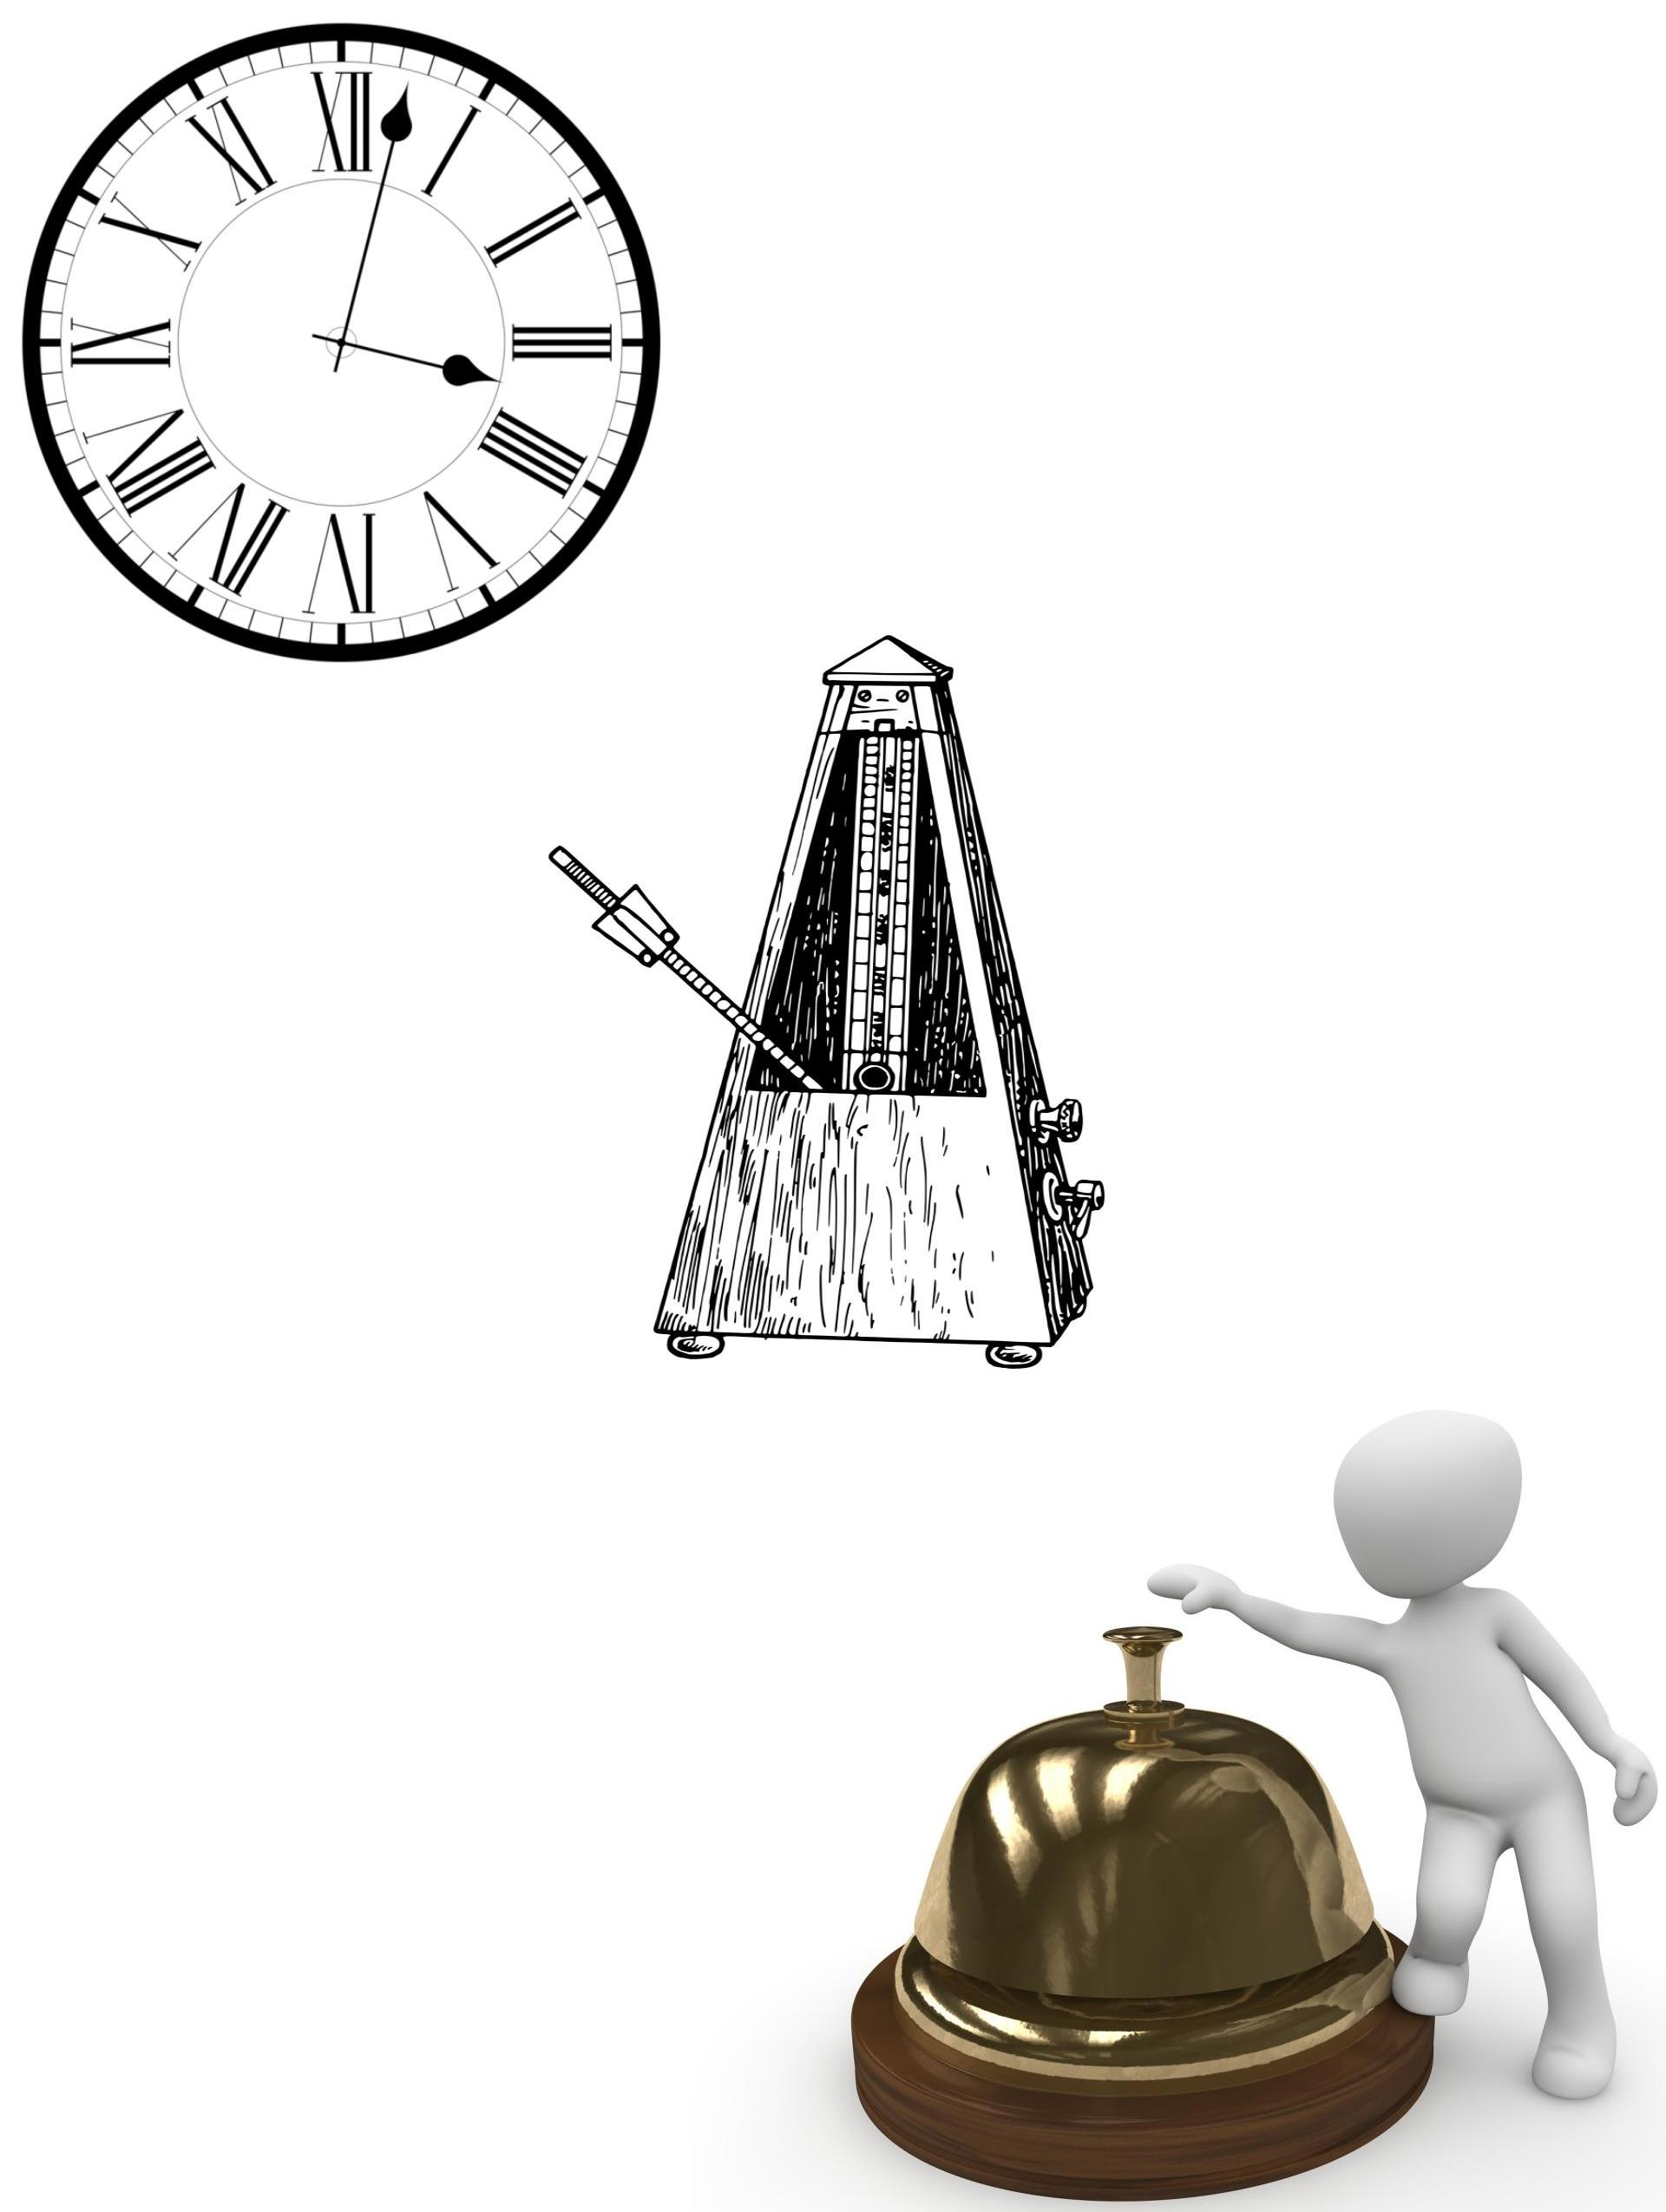
\includegraphics[height=5.5cm]{./Unit-01/img/Taxonomy-When-3_cc0.jpg}}%
  \column[T]{0.70\textwidth}
   \begin{itemize}[<+-| alert@+>]
   \item Continuously $\Rightarrow$ \TC{continuous-time} control\\
         (e.g., analogue electronics).
   \item \vspace{6mm}At points in time known \emph{a priori} $\Rightarrow$ \TC{discrete-time} control\\
         (e.g. and most typical, ISR for a \TC{periodic} interrupt).
   \item \vspace{6mm}When requested $\Rightarrow$ \TC{event-triggered} control\\
         (e.g., when a signal has changed 
          by more\\ than a given quantity wrt the last\\ control determination).
   \end{itemize}
 \end{columns}
\end{frame}

\begin{frame}\mccz
\frametitleTC{A very simple control taxonomy -- axis 3}
\framesubtitleTC{What is the nature of the control action}
\myPause
 \begin{columns}
  \column[T]{0.25\textwidth}
   \only<2 | handout:0>{\centering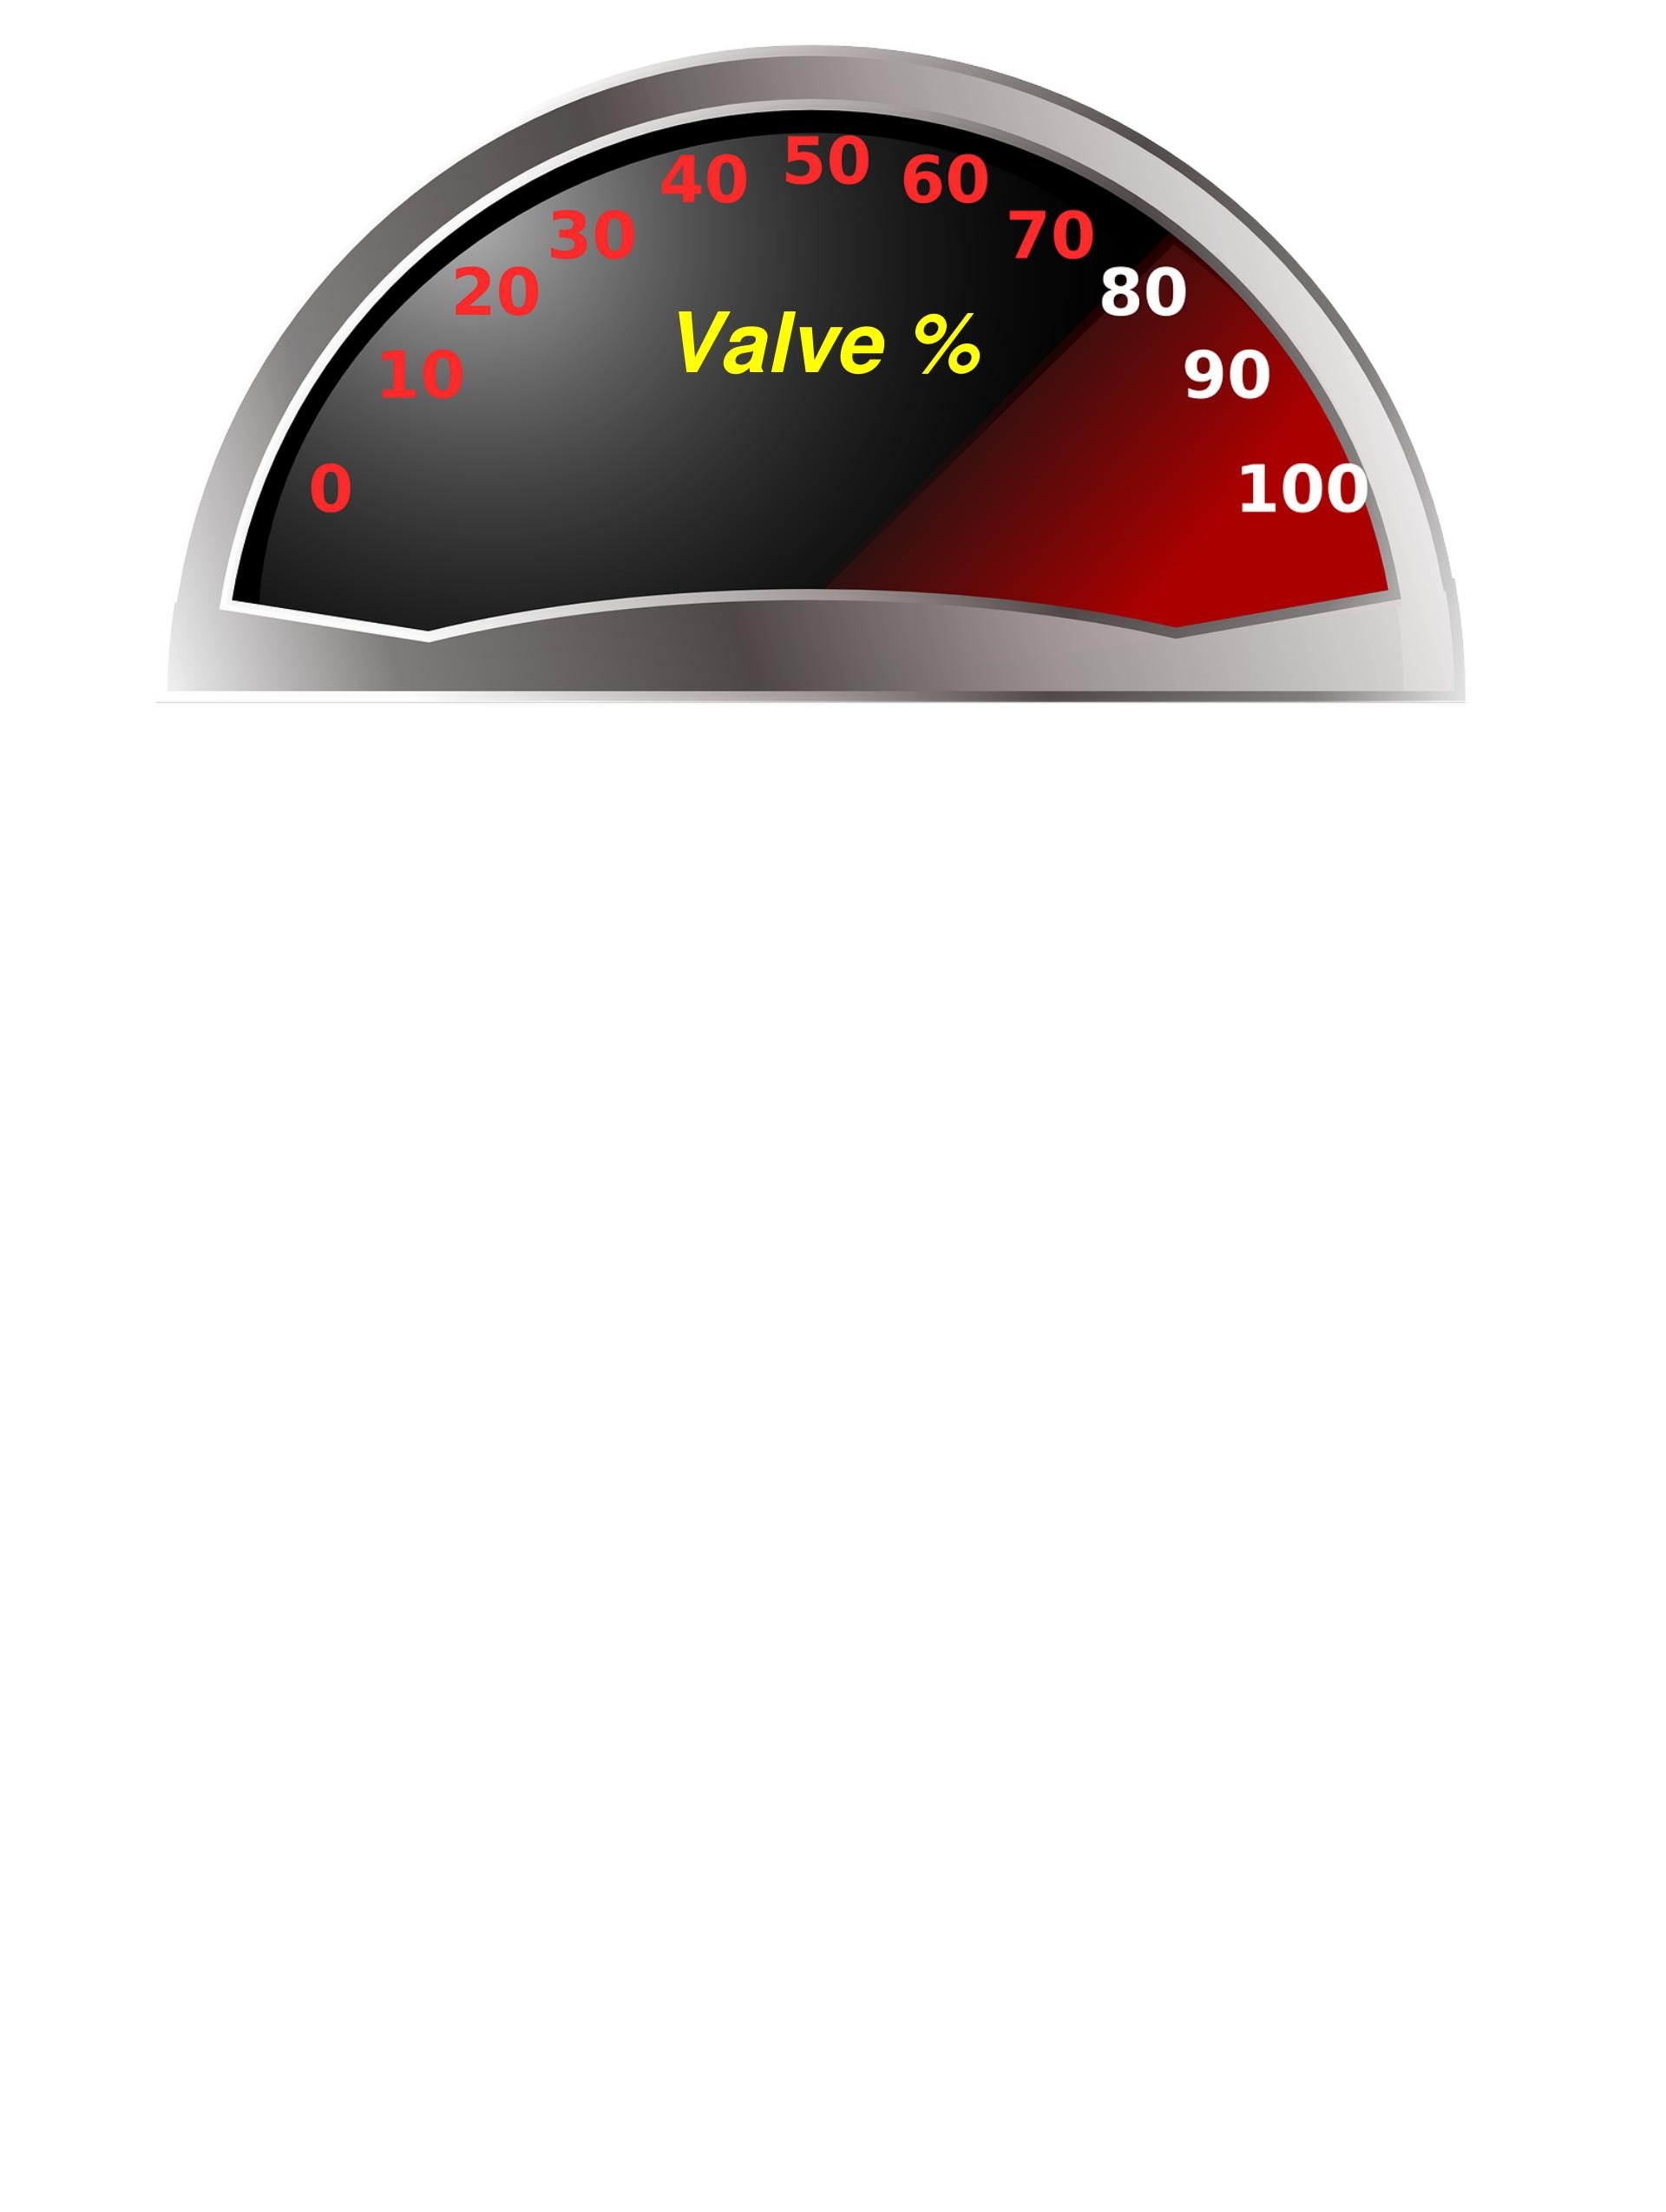
\includegraphics[height=6cm]{./Unit-01/img/Taxonomy-MvsL-1_cc0.jpg}}%
   \only<3-           >{\centering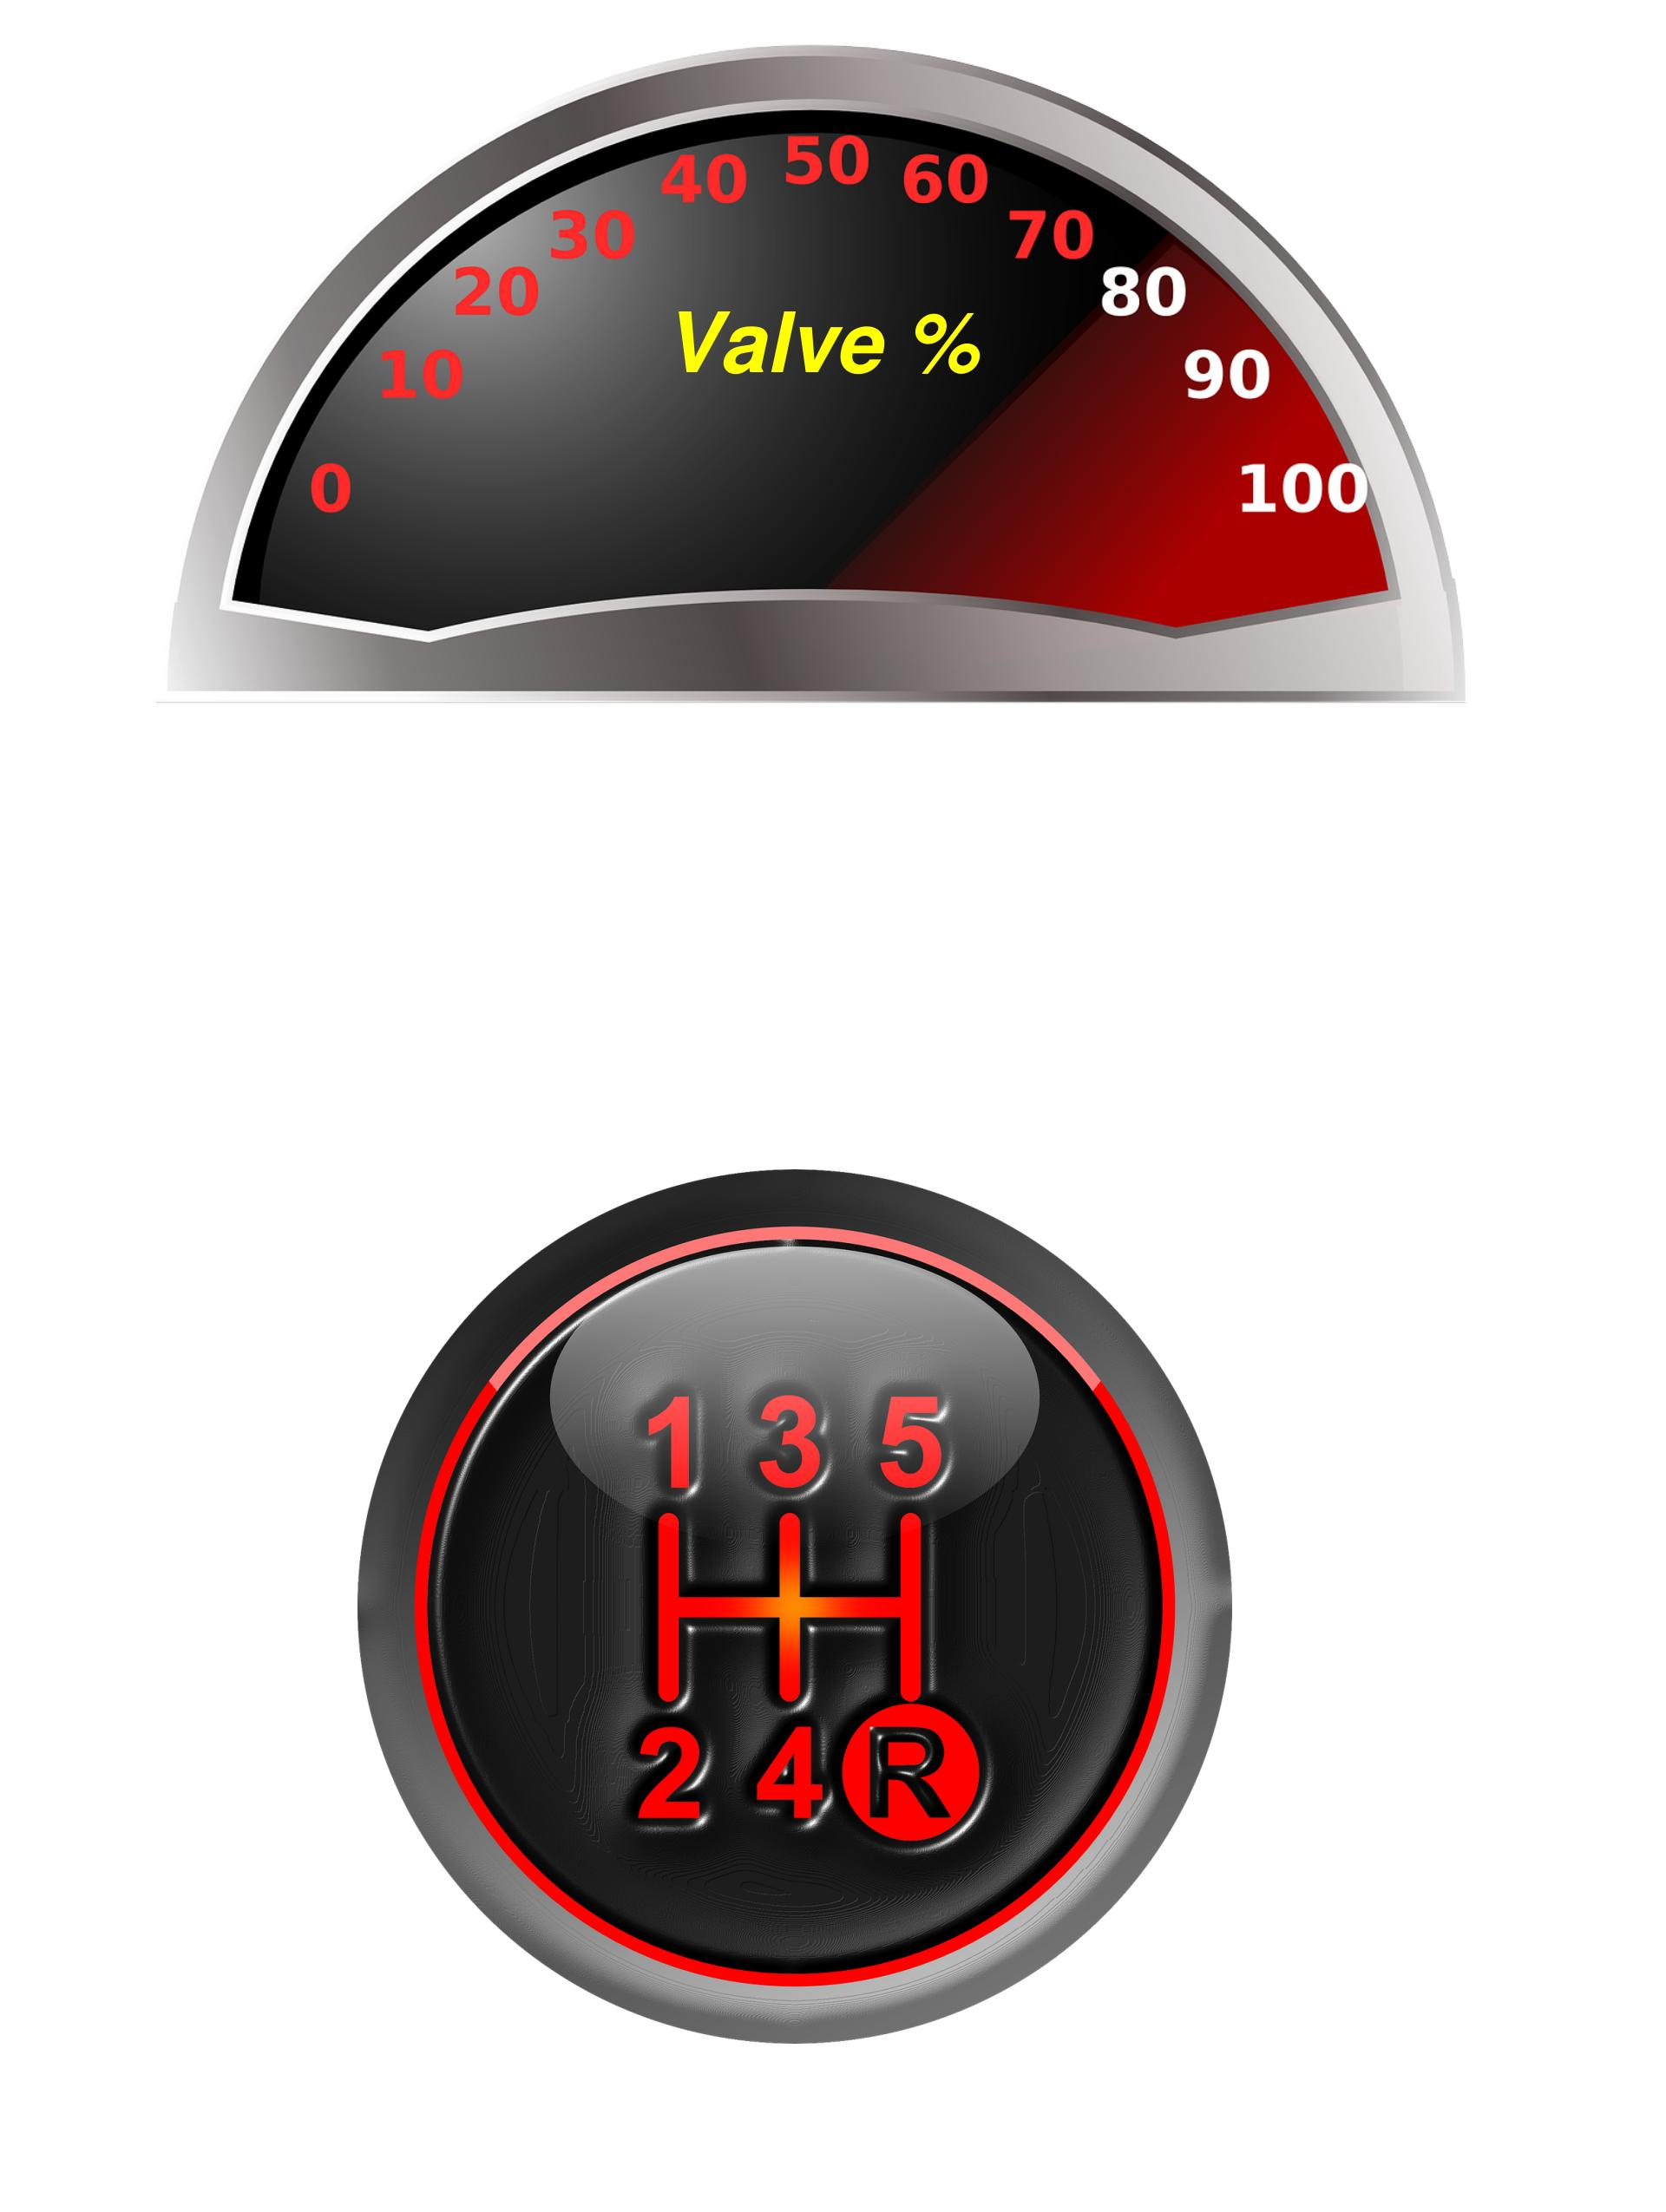
\includegraphics[height=6cm]{./Unit-01/img/Taxonomy-MvsL-2_cc0.jpg}}%
  \column[T]{0.70\textwidth}
   \begin{itemize}[<+-| alert@+>]
   \item Numeric, possibly quantised $\Rightarrow$ \TC{modulating} control\\
         (e.g., valve opening from 0 to 100\%,\\
         motor supply voltage from 0 to 24V in 0.1V steps,...);
         NOTE: \underline{any} such action has lower/upper bounds\\
         owing to physics.
   \item \vspace{10mm}Lexical ($\sim$bool/enum) $\Rightarrow$ \TC{logic} control\\
         (e.g., heater on/off,\\
          gear=\{reverse,neutral,1..5\},\\
          motor dir= \{forward,stop,backward\},...).
   \end{itemize}
 \end{columns}
\end{frame}

\begin{frame}[fragile]
\frametitleTC{Summarising}
\framesubtitleTC{brutally indeed}
\myPause
 \begin{itemize}[<+-| alert@+>]
 \item Controller:\\
         \begin{verbatim}
 type                     = {modulating,logic}
 timing                   = {continuous,discrete,event_triggered}
 connection_with_system   = {open-loop,closed_loop}
 disturbance_compensation = {present,absent}
         \end{verbatim}
 \item \vspace{-5mm}There are corner cases to this taxonomy, but for our purpose we can safely\\
       neglect them.
 \item In complex systems, controllers of different nature co-exist.
 \item \vfill To design and assess a controller, we need a modelling formalism.
 \item To make problems tractable, this formalism must also fit\\
       the controlled system.
 \item We thus move to the concept of \TC{dynamic system}.
 \end{itemize}
\end{frame}


\section{Dynamic systems}
\subsection{}

\begin{frame}\mccz
\frametitleTC{Foreword}
\framesubtitleTC{on how we shall proceed given the breadth of the subject}
\myPause
 \begin{columns}
  \column[T]{0.35\textwidth}
   \only<2 | handout:0>{\centering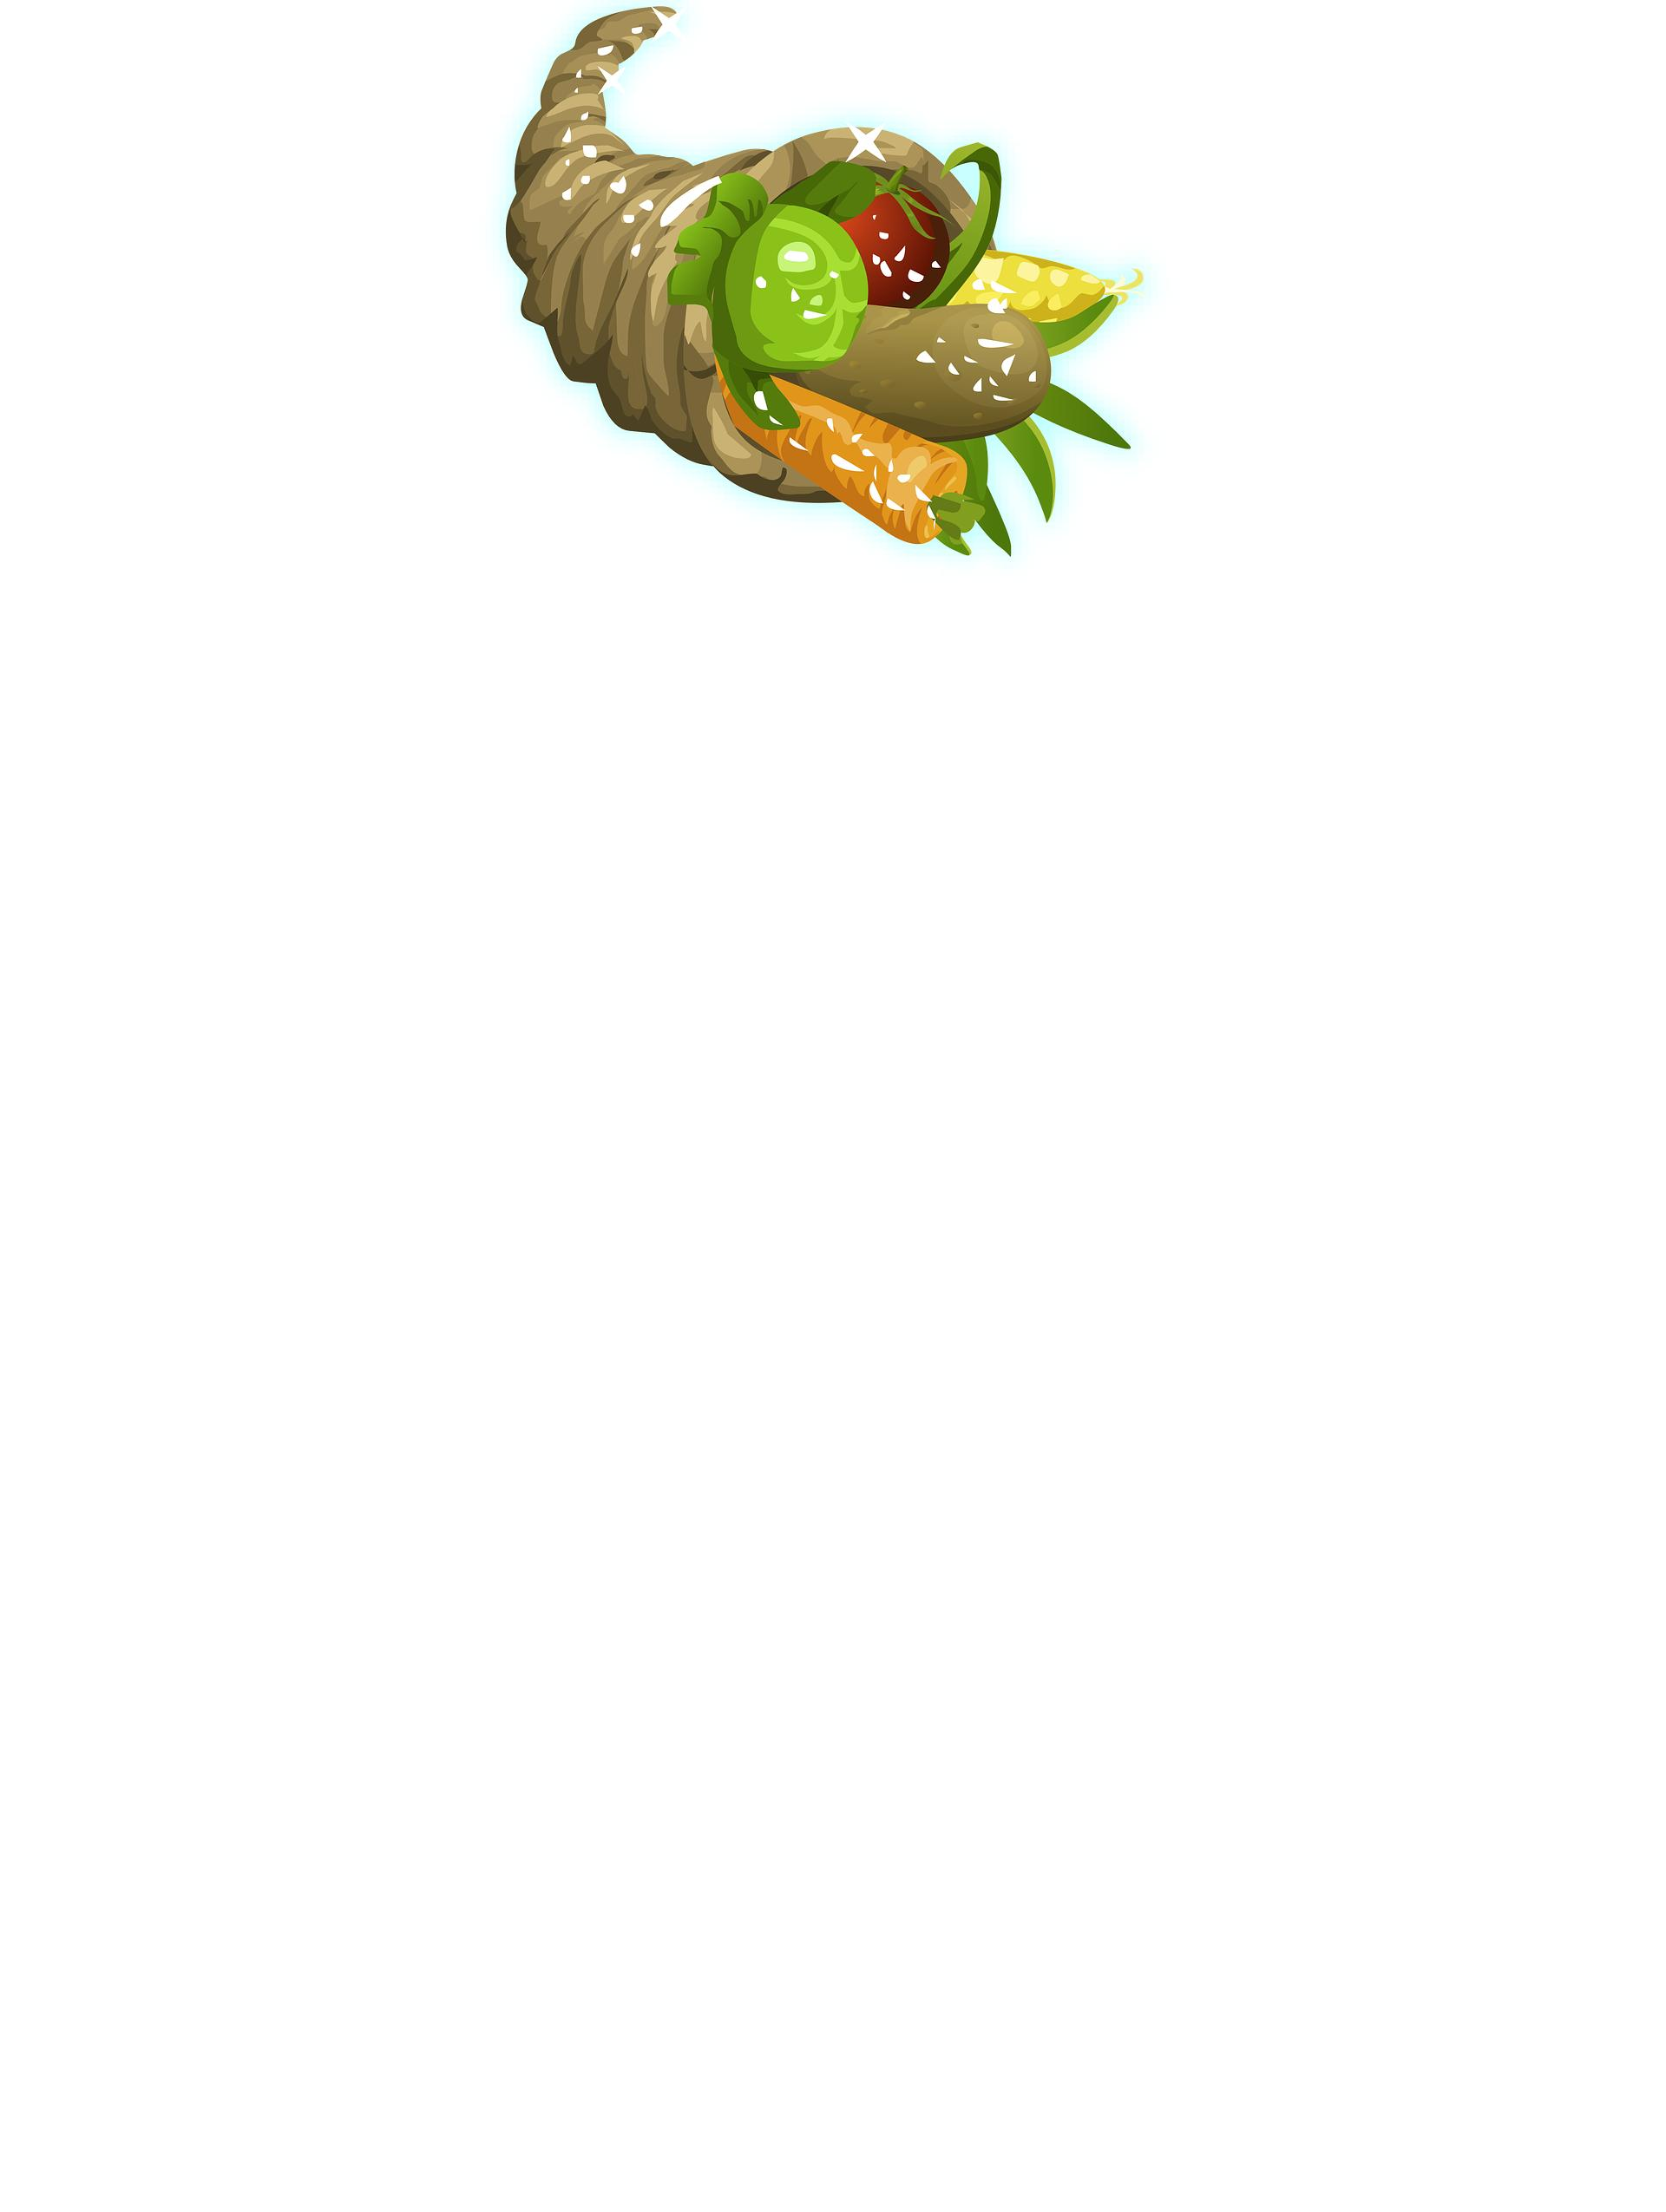
\includegraphics[height=6cm]{./Unit-01/img/DynSys-Variety-1_cc0.jpg}}%
   \only<3 | handout:0>{\centering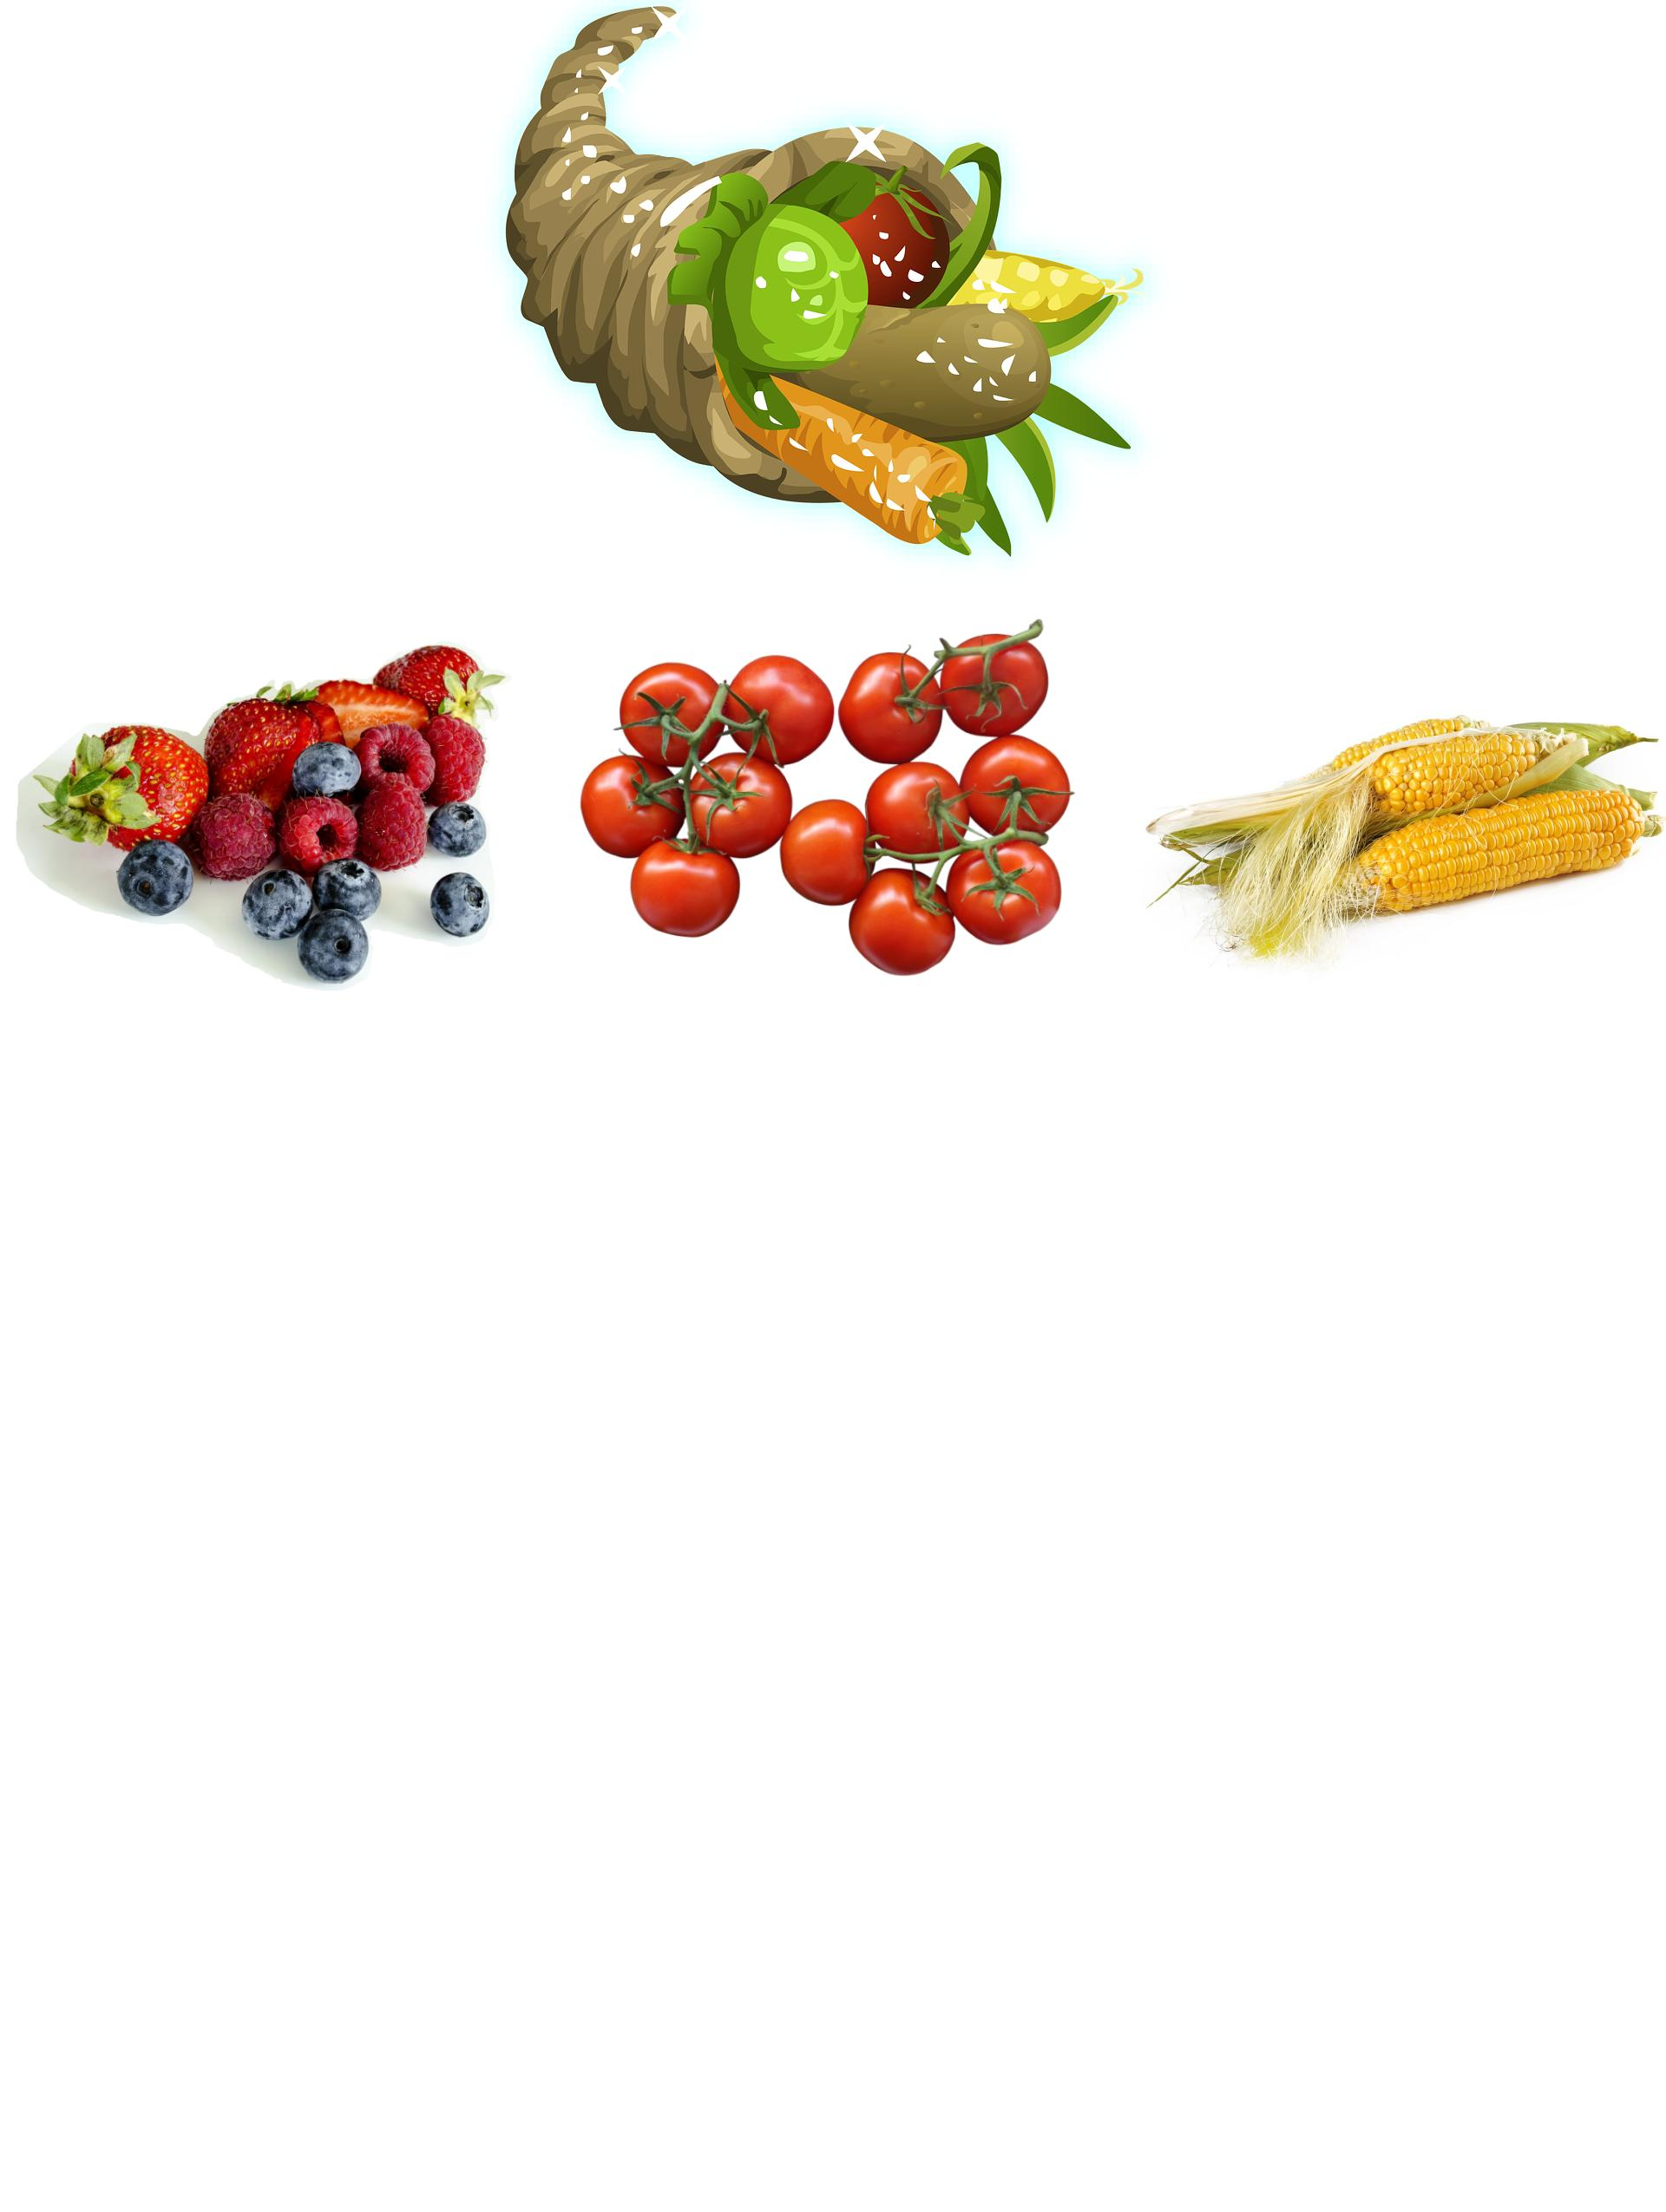
\includegraphics[height=6cm]{./Unit-01/img/DynSys-Variety-2_cc0.jpg}}%
   \only<4 | handout:0>{\centering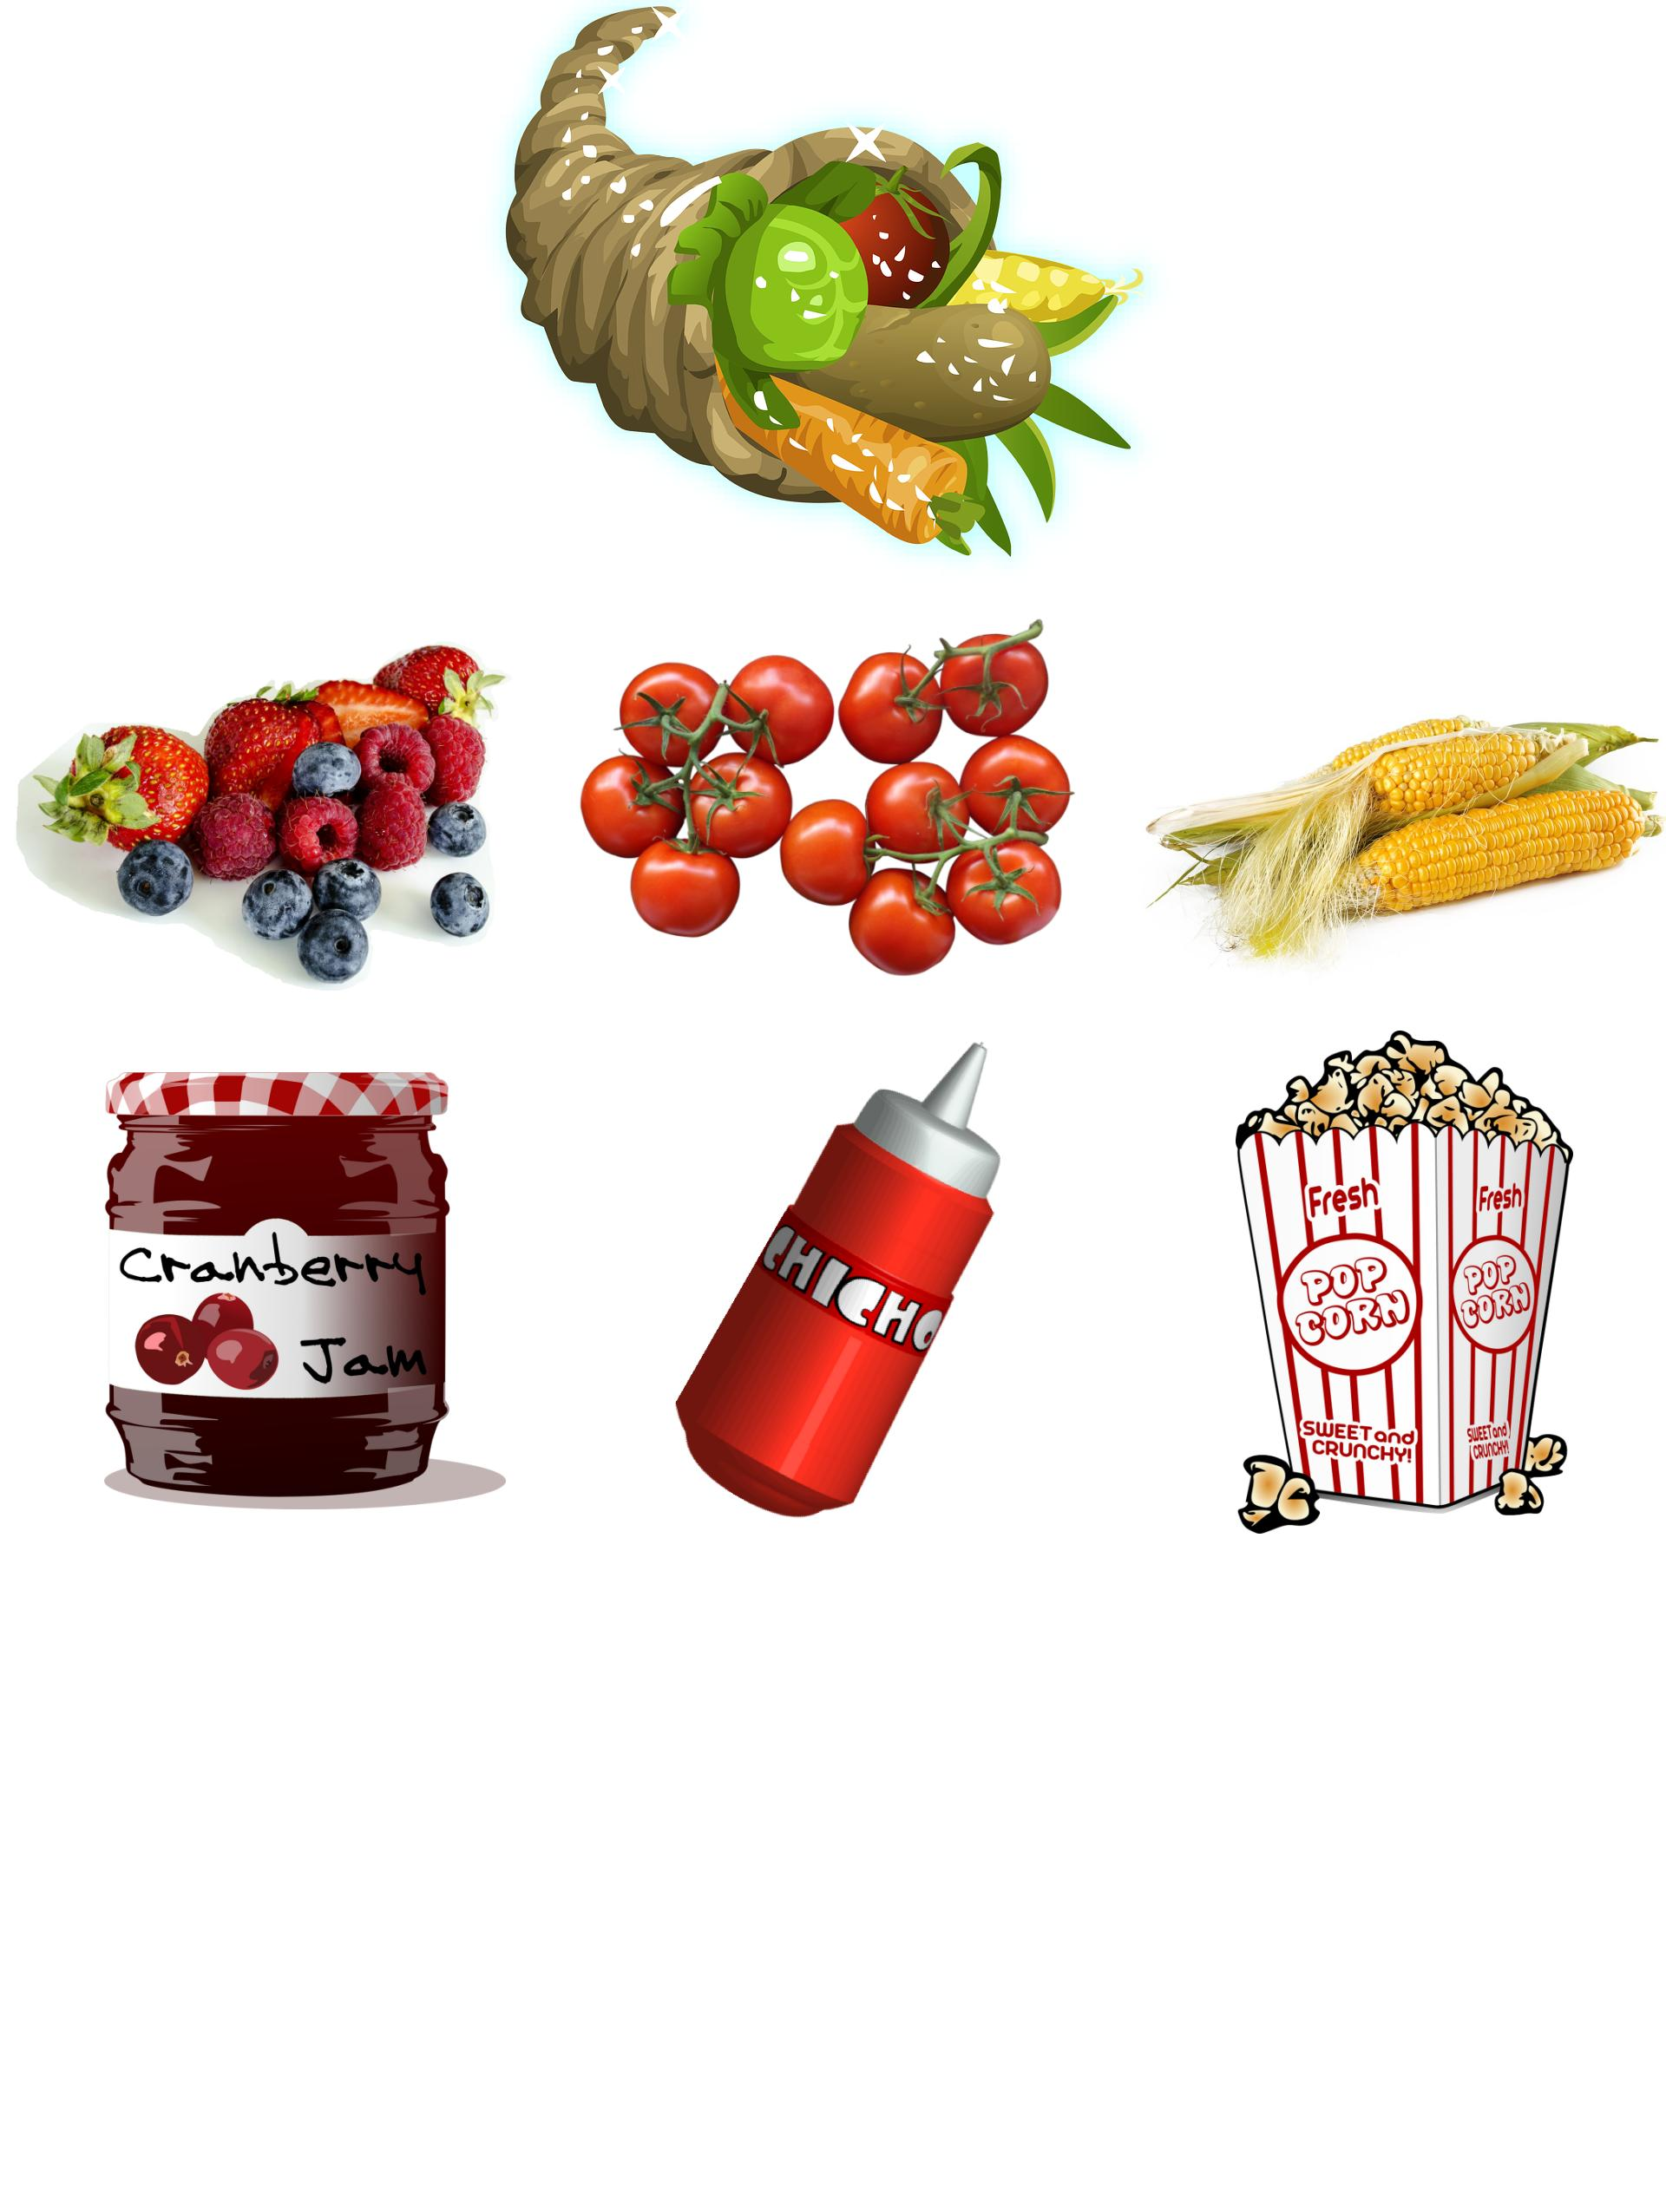
\includegraphics[height=6cm]{./Unit-01/img/DynSys-Variety-3_cc0.jpg}}%
   \only<5-           >{\centering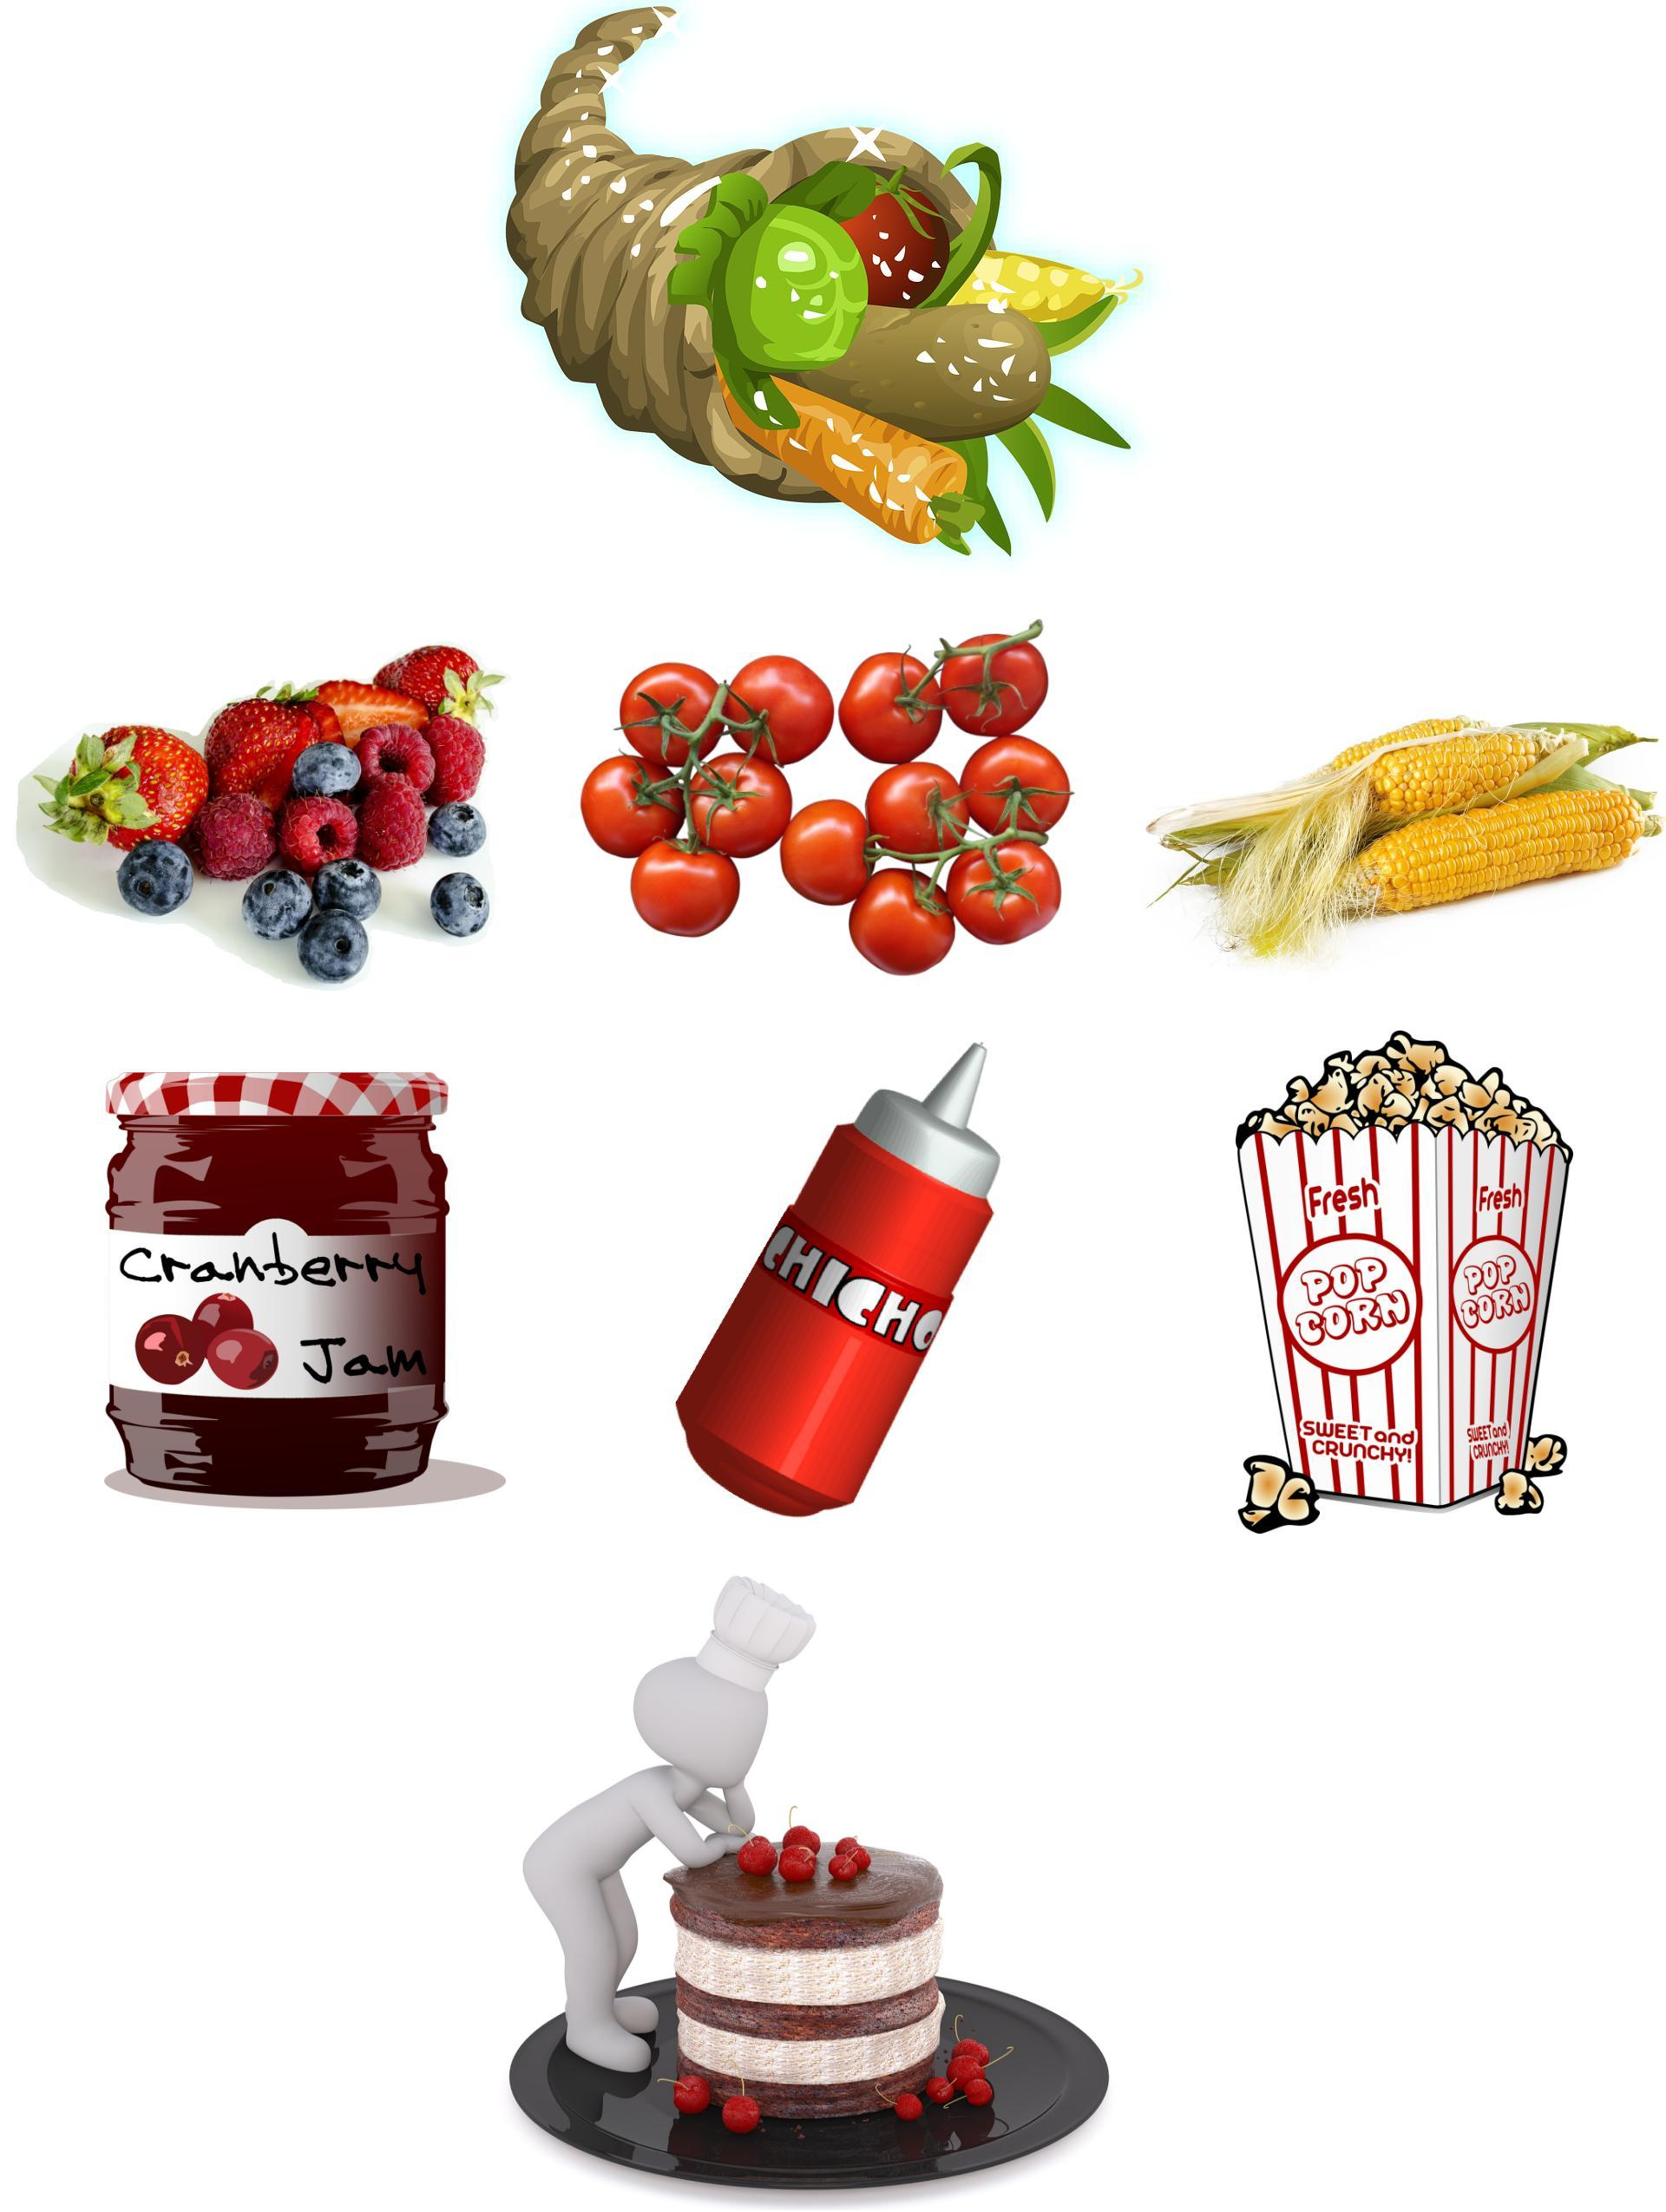
\includegraphics[height=6cm]{./Unit-01/img/DynSys-Variety-4_cc0.jpg}}%
  \column[T]{0.65\textwidth}
   \begin{itemize}[<+-| alert@+>]
   \item We shall state the \underline{general idea} of dynamic system,
   \item \vspace{8mm}then specialise to a few types of interest,
   \item \vspace{8mm}then see what control problems they fit,
   \item \vspace{8mm}and finally restrict to one type\\
         for the purpose of our activity.
   \end{itemize}
 \end{columns}
\end{frame}

\begin{frame}
\frametitleTC{Dynamic system}
\framesubtitleTC{General definition}
\myPause
 \begin{center}
  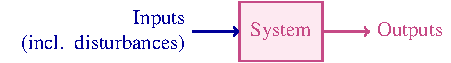
\includegraphics[width=0.6\columnwidth]{./Unit-01/img/DynSys-GenericSystem.pdf}
  \myPause
 \end{center}
 \begin{itemize}[<+-| alert@+>]
 \item Suppose you know the values that the inputs have NOW.
 \item Can you tell which is NOW the values of the outputs?
 \item \vfill If so, the system is \TC{non dynamic}, otherwise it is \TC{dynamic.}
 \item Let us see some examples.
 \end{itemize}
\end{frame}

\begin{frame}
\frametitleTC{Dynamic system}
\framesubtitleTC{Introductory examples (1/3)}
\myPause
 \begin{itemize}[<+-| alert@+>]
 \item \textbf{Example 1}
       \begin{itemize}[<+-| alert@+>]
       \item[] \begin{tabular}{lll}
                System  &: & resistor of resistance $R$.\\
                Input   &: & applied voltage $V(t)$.\\
                Output  &: & flowing current $I(t)$.
               \end{tabular}
       \item \vspace{1mm}At time $\overline{t}$ the input is $V(\overline{t})=\overline{V}$; can you tell what
             the output $I(\overline{t})$ is?
       \item Yes, we have $I(\overline{t})=\overline{V}/R$.
       \item[] $\Rightarrow$ This system is non dynamic. 
       \end{itemize}
 \item \vfill\textbf{Example 2}
       \begin{itemize}[<+-| alert@+>]
       \item[] \begin{tabular}{lll}
                System  &: & water tank with inlet pump and outlet valve at the bottom.\\
                Inputs  &: & pump flowrate, valve opening.\\
                Output  &: & outlet flowrate.
               \end{tabular}
       \item \vspace{1mm}At time $\overline{t}$ we know the inlet pump flowrate and the outlet valve \\
             opening; can you tell what the output (outlet flowrate) is?
       \item No (it depends on valve opening and bottom pressure, i.e., level).
       \item[] $\Rightarrow$ This system is dynamic. 
       \end{itemize}
 \end{itemize}
\end{frame}

\begin{frame}
\frametitleTC{Dynamic system}
\framesubtitleTC{Introductory examples (2/3)}
\myPause
 \begin{itemize}[<+-| alert@+>]
 \item \textbf{Example 3}
       \begin{itemize}[<+-| alert@+>]
       \item[] \begin{tabular}{lll}
                System  &: & bus.\\
                Input   &: & $\Delta p(k)$, passengers on minus passengers off at stop $k$.\\
                Output  &: & passengers aboard when leaving stop $k$.
               \end{tabular}
       \item \vspace{1mm}At stop $k$ three passengers get on and two off, hence $\Delta p(k)=1$; can you tell\\
             how many passengers are aboard when leaving stop $k$?
       \item No (I should know how many were aboard before arriving at stop $k$).
       \item[] $\Rightarrow$ This system is dynamic. 
       \end{itemize}
 \end{itemize}
\end{frame}

\begin{frame}
\frametitleTC{Dynamic system}
\framesubtitleTC{Introductory examples (3/3)}
\myPause
 \begin{itemize}[<+-| alert@+>]
 \item \textbf{Example 4} -- note the slight difference
       \begin{itemize}[<+-| alert@+>]
       \item[] \begin{tabular}{lll}
                System  &: & lamp.\\
                Input   &: & button, when pressed the lamp goes on if off and \emph{vice versa}.\\
                Output  &: & lamp status (on/off).
               \end{tabular}
       \item \vspace{1mm}In the last hour we pressed the button 8 times;\\
             can you tell the status of the lamp?
       \item No (I should know the status 1 hour ago, however I can say that now\\
             the status is the same it was 1 hour ago).
       \item[] $\Rightarrow$ This system is dynamic. 
       \end{itemize}
 \end{itemize}
\end{frame}

\begin{frame}
\frametitleTC{Dynamic system}
\framesubtitleTC{Introductory examples -- summary for the dynamic cases}
\myPause
 \begin{itemize}[<+-| alert@+>]
 \item Example 2:
       \begin{itemize}[<+-| alert@+>]
       \item the system evolves in the continuous time,
       \item need to know the present tank level.
       \end{itemize}
 \item Example 3:
       \begin{itemize}[<+-| alert@+>]
       \item the system evolves in steps (stops 1 to last),
       \item need to know the previous bus occupancy.
       \end{itemize}
 \item Example 4:
       \begin{itemize}[<+-| alert@+>]
       \item the system evolves when events occur (no \emph{a priori} idea how many\\
             in a given timespan),
       \item need to know the initial lamp status.
       \end{itemize}
 \item \vfill So in general, to know the outputs, I need to know the inputs\\
       plus the present (or initial, or ``previous'' when applicable)\\
       value of something else.
 \item This "something else" is the system \TC{state.}
 \end{itemize}
\end{frame}

\begin{frame}
\frametitleTC{Classes of dynamic systems}
\framesubtitleTC{No theory, just intuition and abstraction from the examples}
\myPause
 \begin{itemize}[<+-| alert@+>]
 \item Common elements: input, output and \TC{state} (variables).
 \item Two equivalent viewpoints:
       \begin{itemize}[<+-| alert@+>]
       \item \underline{present state} and possibly present input $\Rightarrow$ present output\\
             (in the tank, opening and level now $\Rightarrow$ outlet flow now);
       \item \underline{initial state} and input story $\Rightarrow$ state and output story\\
             (initial level, inflow and opening story $\Rightarrow$ level and outflow story).
       \end{itemize}
 \item \vspace{2mm}General fact: dynamic systems
       \begin{itemize}[<+-| alert@+>]
       \item have memory of the past,
       \item and can respond differently to the same input, because they have a state.
       \end{itemize}
 \item \vfill Revisiting the examples and generalising, we shall now introduce\\
       three classes of dynamic systems:
       \begin{itemize}[<+-| alert@+>]
       \item continuous-time,
       \item discrete-time,
       \item and discrete-events.
       \end{itemize}
 \end{itemize}
\end{frame}

\begin{frame}
\frametitleTC{Continuous-time (CT) dynamic systems}
\myPause
 \begin{itemize}[<+-| alert@+>]
 \item They are made of \TC{differential equations.} Let us see what happens with the tank.
 \item Cylindrical tank of area $A$, fluid of constant density $\rho$, variable level $\ell(t)$
 \item Contained mass $M(t) = \rho A \ell(t)$.
 \item Bottom pressure $p(t) = \rho g \ell(t)$, where $g$ is gravity acceleration.
 \item Derivative of mass with time = inlet flowrate minus outlet flowrate.
 \item Inlet flowrate $w_i(t)$ is an input.
 \item Outlet flowrate $w_o(t)=A_v o(t) \sqrt{\rho p(t)}$, $A_v$ is a valve constant and $o(t)$ the opening.
 \item Valve opening $o(t)$ is an input, while $w_o(t)$ is the system output.
 \item The state is $\ell(t)$ and evolves from the initial value $\ell_0$ at $t=t_0$\\
       according to
       \begin{displaymath}
        \frac{dM(t)}{dt} = \rho A \frac{d\ell(t)}{dt} = w_i(t) - A_v o(t) \sqrt{\rho p(t)}, \quad
        \ell(t_0) = \ell_0.
       \end{displaymath}
 \end{itemize}
\end{frame}

\begin{frame}
\frametitleTC{Continuous-time dynamic systems}
\framesubtitleTC{In general}
\myPause
 \begin{itemize}[<+-| alert@+>]
 \item Input $u(t)$, state $x(t)$ with initial value $x_0$ at $t=t_0$, output $y(t)$;
       \begin{displaymath}
        \left\{\begin{array}{rll}
         \frac{dx(t)}{dt} &= f\left(x(t),u(t),t\right) &\quad \text{[State equation]} \\
         y(t)             &= g\left(x(t),u(t),t\right) &\quad \text{[Output equation]}
        \end{array}\right. \qquad
        x(t_0) = x_0.
       \end{displaymath}
 \item In the following for compactness we shall write $\dot{x}(t)$ to indicate $\frac{dx(t)}{dt}$.
 \item \vfill Enough on these systems for the moment (and for the great\\
       majority of our activity).
 \end{itemize}
\end{frame}

\begin{frame}
\frametitleTC{Discrete-time (DT) dynamic systems}
\myPause
 \begin{itemize}[<+-| alert@+>]
 \item They are made of \TC{difference equations.} Let us see what happens with the bus.
 \item Passengers after leaving stop $k$ = passengers before arriving at stop $k$ plus passengers on
       minus passengers off at stop $k$.
 \item Denote by $p(k)$ the passengers \underline{after} stop $k$ and by $\Delta p(k)$ the net variation
       or passengers (on minus off) at stop $k$, and we have
       \begin{displaymath}
        p(k) = p(k-1)+\Delta p(k).
       \end{displaymath}
 \end{itemize}
\end{frame}

\begin{frame}
\frametitleTC{Discrete-time dynamic systems}
\framesubtitleTC{In general}
\myPause
 \begin{itemize}[<+-| alert@+>]
 \item The integer $k$ is the ``time index'': it can really be time-related if it corresponds to the elapsing
       of a fixed period (giving rise to \TC{sampled-data} systems) or just count the evolution steps (bus stops,...).
 \item Input $u(t)$k, state $x(k)$ with initial value $x_0$ at $k=k_0$, output $y(k)$;
       \begin{displaymath}
        \left\{\begin{array}{rll}
         x(k) &= f\left(x(k-1),u(k-1),k\right) &\quad \text{[State equation]} \\
         y(k) &= g\left(x(k-1),u(k-1),k\right) &\quad \text{[Output equation]}
        \end{array}\right. \qquad
        x(k_0) = x_0.
       \end{displaymath}
 \item Read: at each step
       \begin{itemize}[<+-| alert@+>]
       \item I take the old state an the old input, and compute the new state,
       \item then I take the new state and the new input, and compute\\
             the new output.
       \end{itemize}
 \end{itemize}
\end{frame}

\begin{frame}
\frametitleTC{LTI (Linear, Time-Invariant) dynamic systems -- both CT and DT}
\framesubtitleTC{A specific but extremely useful subclass}
\myPause
 \begin{itemize}[<+-| alert@+>]
 \item \vspace{2mm}Linear: functions $f(\cdot,\cdot,\cdot)$ and  $g(\cdot,\cdot,\cdot)$ linear in $x$ and $u$.
 \item Time-invariant: $f$ and $g$ do not depend explicitly on $t$ (CT case) or $k$ (DT case).
 \item Input $u(t|k)$, state $x(t|k)$ with initial value $x_0$ at $t|k=t_0|k_0$, output $y(t|k)$;
       \begin{displaymath}
         \begin{array}{lll}
          \text{CT case:} & 
          \left\{\begin{array}{rll}
           \dot{x}(t) &= Ax(t)+bu(t) \\
           y(t)       &= cx(t)+du(t)
          \end{array}\right. &
          x(0) = x_0 \\ \\
          \text{DT case:} & 
          \left\{\begin{array}{rll}
           x(k) &= Ax(k-1)+bu(k-1) \\
           y(k) &= cx(k)+du(k)
          \end{array}\right. &
          x(0) = x_0
         \end{array}
        \end{displaymath}
 \item \vfill The time origin is zero because the system is time-invariant (TI).
 \item $A$, $b$, $c$ and $d$ are matrices of convenient dimensions. 
 \end{itemize}
\end{frame}

\begin{frame}
\frametitleTC{Discrete-event dynamic systems}
\myPause
 \begin{itemize}[<+-| alert@+>]
 \item Not driven by time but rather by events.
 \item Represented as automata, Petri nets, and the like.
 \item Example automaton for the lamp:
       \begin{center}
        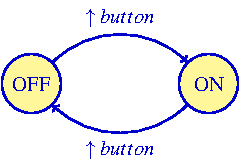
\includegraphics[width=0.30\columnwidth]{./Unit-01/img/DynSys-LampAutomaton.pdf}
       \end{center}
 \item In our activity we are not addressing this kind of systems.
 \item Let us move to a \emph{rough} (system class)--(control problem) pairing.
 \end{itemize}
\end{frame}

\begin{frame}
\frametitleTC{Dynamic systems classes and control problems}
\framesubtitleTC{...this time looking at computers -- just an overview to stimulate discussion}
\myPause
 \begin{itemize}[<+-| alert@+>]
 \item Group 1 -- problems directly related to physics \emph{stricto sensu}:
       \begin{itemize}[<+-| alert@+>]
       \item typical example -- CPU temperature;
       \item system model -- continuous-time dynamic system;
       \item controller design -- as continuous-time system, then converted to discrete-time\\
             to become control \TC{code}.
       \end{itemize}
 \item Group 2 -- problems not in group 1 where requirements are translatable into desired behaviours
       of signals (reference or admissible range):
       \begin{itemize}[<+-| alert@+>]
       \item typical example -- deadline enforcement, obtained by tracking a desired completion\\
             that reaches 100\% by the deadline (\underline{many} problems can be formulated\\
             this way or analogously);
       \item system model -- discrete-time dynamic system;
       \item controller design -- as discrete-time system, then code.
       \end{itemize}
 \item Group 3 -- anything else:
       \begin{itemize}[<+-| alert@+>]
       \item mixed design strategy (not in the scope of our activity),
       \item or not suited for a control-theoretical design.
       \end{itemize}
 \end{itemize}
\end{frame}


\section{Conclusions}
\subsection{}

\begin{frame}
\frametitleTC{Conclusions}
\framesubtitleTC{Recap and lessons learnt (1/3)}
\myPause
 \begin{itemize}[<+-| alert@+>]
 \item Control is \TC{governing a phenomenon} (physical or not).
 \item This means determining \TC{actions} on that phenomenon, based on \TC{requirements}\\
       and possibly \TC{measurements}.
 \item Major issues are exogenous actions -- or \TC{disturbances} -- and \TC{uncertainty},\\
       i.e., only partial knowledge of the controlled system.
 \item Quite often a control problem can be formulated in terms of signals,\\
       i.e., as \TC{tracking a reference} and/or \TC{rejecting disturbances}.
 \end{itemize}
\end{frame}

\begin{frame}
\frametitleTC{Conclusions}
\framesubtitleTC{Recap and lessons learnt (2/3)}
\myPause
 \begin{itemize}[<+-| alert@+>]
 \item A controller may or may not know the effects of its action on the controlled system, giving rise to
       \TC{closed-loop} (or \TC{feedback}) versus \TC{open-loop} control.
 \item A controller can operate in the continuous time, but in computing systems this is\\
       practically never the case;
 \item hence for us a controller is a piece of code, invoked either periodically or based\\
       on events, giving rise to \TC{discrete-time} versus \TC{event-based} control.
 \item Control signals can be \TC{numeric} or \TC{lexical}, corresponding to \TC{modulating}\\
       versus \TC{logic} control.
 \item Control problems are posed and treated with reference to one\\
       or more classes of \TC{dynamic systems}. 
 \end{itemize}
\end{frame}

\begin{frame}
\frametitleTC{Conclusions}
\framesubtitleTC{Recap and lessons learnt (3/3)}
\myPause
 \begin{itemize}[<+-| alert@+>]
 \item Dynamic systems have a \TC{state}, hence they
       \begin{itemize}[<+-| alert@+>]
       \item remember the past,
       \item or -- equivalently -- their initial condition,
       \item and thus \TC{can produce different outputs in response to the same input}...
       \item ...without however being time-varying or ``adaptive'' (remember this remark!).
       \end{itemize}
 \item We have seen some classes of dynamic systems.
 \item In the following we shall concentrate on LTI ones, almost exclusively\\
       in the DT domain. 
 \end{itemize}
\end{frame}

\section{}
{
\setbeamertemplate{headline}{
  \begin{beamercolorbox}[wd=\paperwidth,ht=4.2ex,dp=1.5ex]{palette quaternary}
  \end{beamercolorbox}
  }
\setbeamertemplate{footline}{
  \begin{beamercolorbox}[wd=\paperwidth,ht=2.2ex,dp=1.5ex]{palette quaternary}
  \end{beamercolorbox}
  }
\begin{frame}[noframenumbering]
 \vspace{20mm}\Huge{Discussion open}
\end{frame}
}







